\documentclass[oneside,senior,etd]{BYUPhysForDegree}

\usepackage[utf8]{inputenc}
\usepackage{rotating} 
\usepackage{caption}

\usepackage[russian]{babel}
\usepackage{amsfonts} % Пакеты для математических символов и теорем
\usepackage{amstext}
\usepackage{amssymb}
\usepackage{amsthm}
\usepackage{graphicx} % Пакеты для вставки графики
\usepackage{subfig}
\usepackage{color}
\usepackage[unicode]{hyperref}
\usepackage[nottoc]{tocbibind} % Для того, чтобы список литературы отображался в оглавлении
\usepackage{algorithmic} % Для записи алгоритмов в псевдокоде
\usepackage{algorithm}
\usepackage{verbatim} % Для вставок заранее подготовленного текста в режиме as-is
\usepackage{listings}
\usepackage{array}
\usepackage[numbers]{natbib}
\newcommand{\citeappendix}[2]{[\citenum{#1}, #2]}


\usepackage{commath}
\newcommand\Tau{\mathcal{T}}
\newcommand{\R}{\mathbb{R}}
\usepackage{color}
\usepackage[colorinlistoftodos, prependcaption]{todonotes}
\usepackage{multirow}
\newcommand*{\MyIndent}{\hspace*{0.2cm}}%

\Chair{Кафедра автоматизации систем вычислительных комплексов}
\Lab{~}
\Year{2026}
  \Month{Май}
  \City{Москва}
  \AuthorText{Автор}
  \Author{Гоцкало Максим Олегович}
  \AuthorEng{}
  \AcadGroup{321}

  \TitleTop{Детерминированные алгоритмы построения}
  \TitleMiddle{многопроцессорного расписания}
  \TitleBottom{с ограничением на объем памяти} % leave empty if you don't need it
  \TitleTopEng{}
  \TitleBottomEng{} % leave empty if you don't need it  
  %\docname{Курсовая работа}
  \docname{Курсовая работа}
  %\docname{Магистерская диссертация}
  \Advisor{Балашов Василий Викторович}
  \AdvisorDegree{к.ф.-м.н., с.н.с.}

\Abstract{Здесь будет аннотация}



%%%% DON'T change this. It is here because .sty does not support cyrillic cp properly %%%%
\University{Московский государственный университет имени М.В.Ломоносова}
\Faculty{Факультет вычислительной математики и кибернетики}
\GrText{гр.}
\AdvisorText{Научный руководитель}
\AbstractText{Аннотация}


\begin{document}
\fixmargins
\makepreliminarypages

\oneandhalfspace

\tableofcontents


\anonsection{Введение}
\label{sec:0_vvedenie} \index{0_vvedenie}

В современных вычислительных системах, особенно во встраиваемых и высокопроизводительных приложениях, критически важным ресурсом часто является оперативная память. При выполнении набора работ (задач), связанных отношением частичного порядка (граф потока данных), каждая работа может порождать один или несколько выходных буферов, которые занимают память до момента, когда все их потребители завершат выполнение. Ограниченность памяти накладывает дополнительные условия на допустимость расписания: в любой момент времени суммарный объём активных буферов не должен превышать заданного предела $M$. Требуется построить такое расписание (распределение работ по процессорам и порядок их выполнения), чтобы общая длительность (makespan) была минимальной.

Данная задача возникает, например, при проектировании систем цифровой обработки сигналов (ЦОС), где каждый вычислительный модуль (например, БПФ, фильтр) потребляет и производит массивы данных фиксированного размера, а память является ограничивающим фактором~\cite{Ershov1962}. Аналогичные проблемы характерны для научных конвейерных вычислений (scientific workflows), где промежуточные результаты могут иметь большой объём~\cite{BalashovBasalov2025}. Многопроцессорное планирование с учётом ограничений памяти является NP-трудной задачей, поэтому практические методы делятся на две категории: точные (например, сведение к целочисленному линейному программированию) и приближённые (например, жадные эвристики).

В работе~\cite{Savitsky2023} предложен жадный алгоритм для многопроцессорного списочного планирования с ограничением на долю межпроцессорных передач; в настоящей работе этот алгоритм адаптирован для учёта памяти, а также разработана новая эвристика STS (Smallest Time Space), учитывающая не только длительность работы, но и объём создаваемых ею буферов и длительности потребителей. Для малых графов (до 21 вершины) выполнено сведение к задаче ЦЛП по схеме, аналогичной описанной в работе~\cite{Senyushkina2025} для однопроцессорного случая, с добавлением переменных, моделирующих пересечение интервалов активности буферов. Выбор решателя SCIP обоснован в~\cite{Senyushkina2025}.

На рис.~\ref{fig:graph_example} приведён пример графа работ, а на~\ref{fig:shed_example} - двух возможных расписаний (построенных жадным алгоритмом и оптимального). Видно, что оптимальное расписание позволяет лучше использовать память и процессоры, избегая длительных простоев.\\

Для описанной выше задачи в работе представлены и исследованы жадные алгоритмы с двумя различными эвристиками, а также подход на основе целочисленного линейного программирования.\\

\begin{figure}[h]
	\centering
	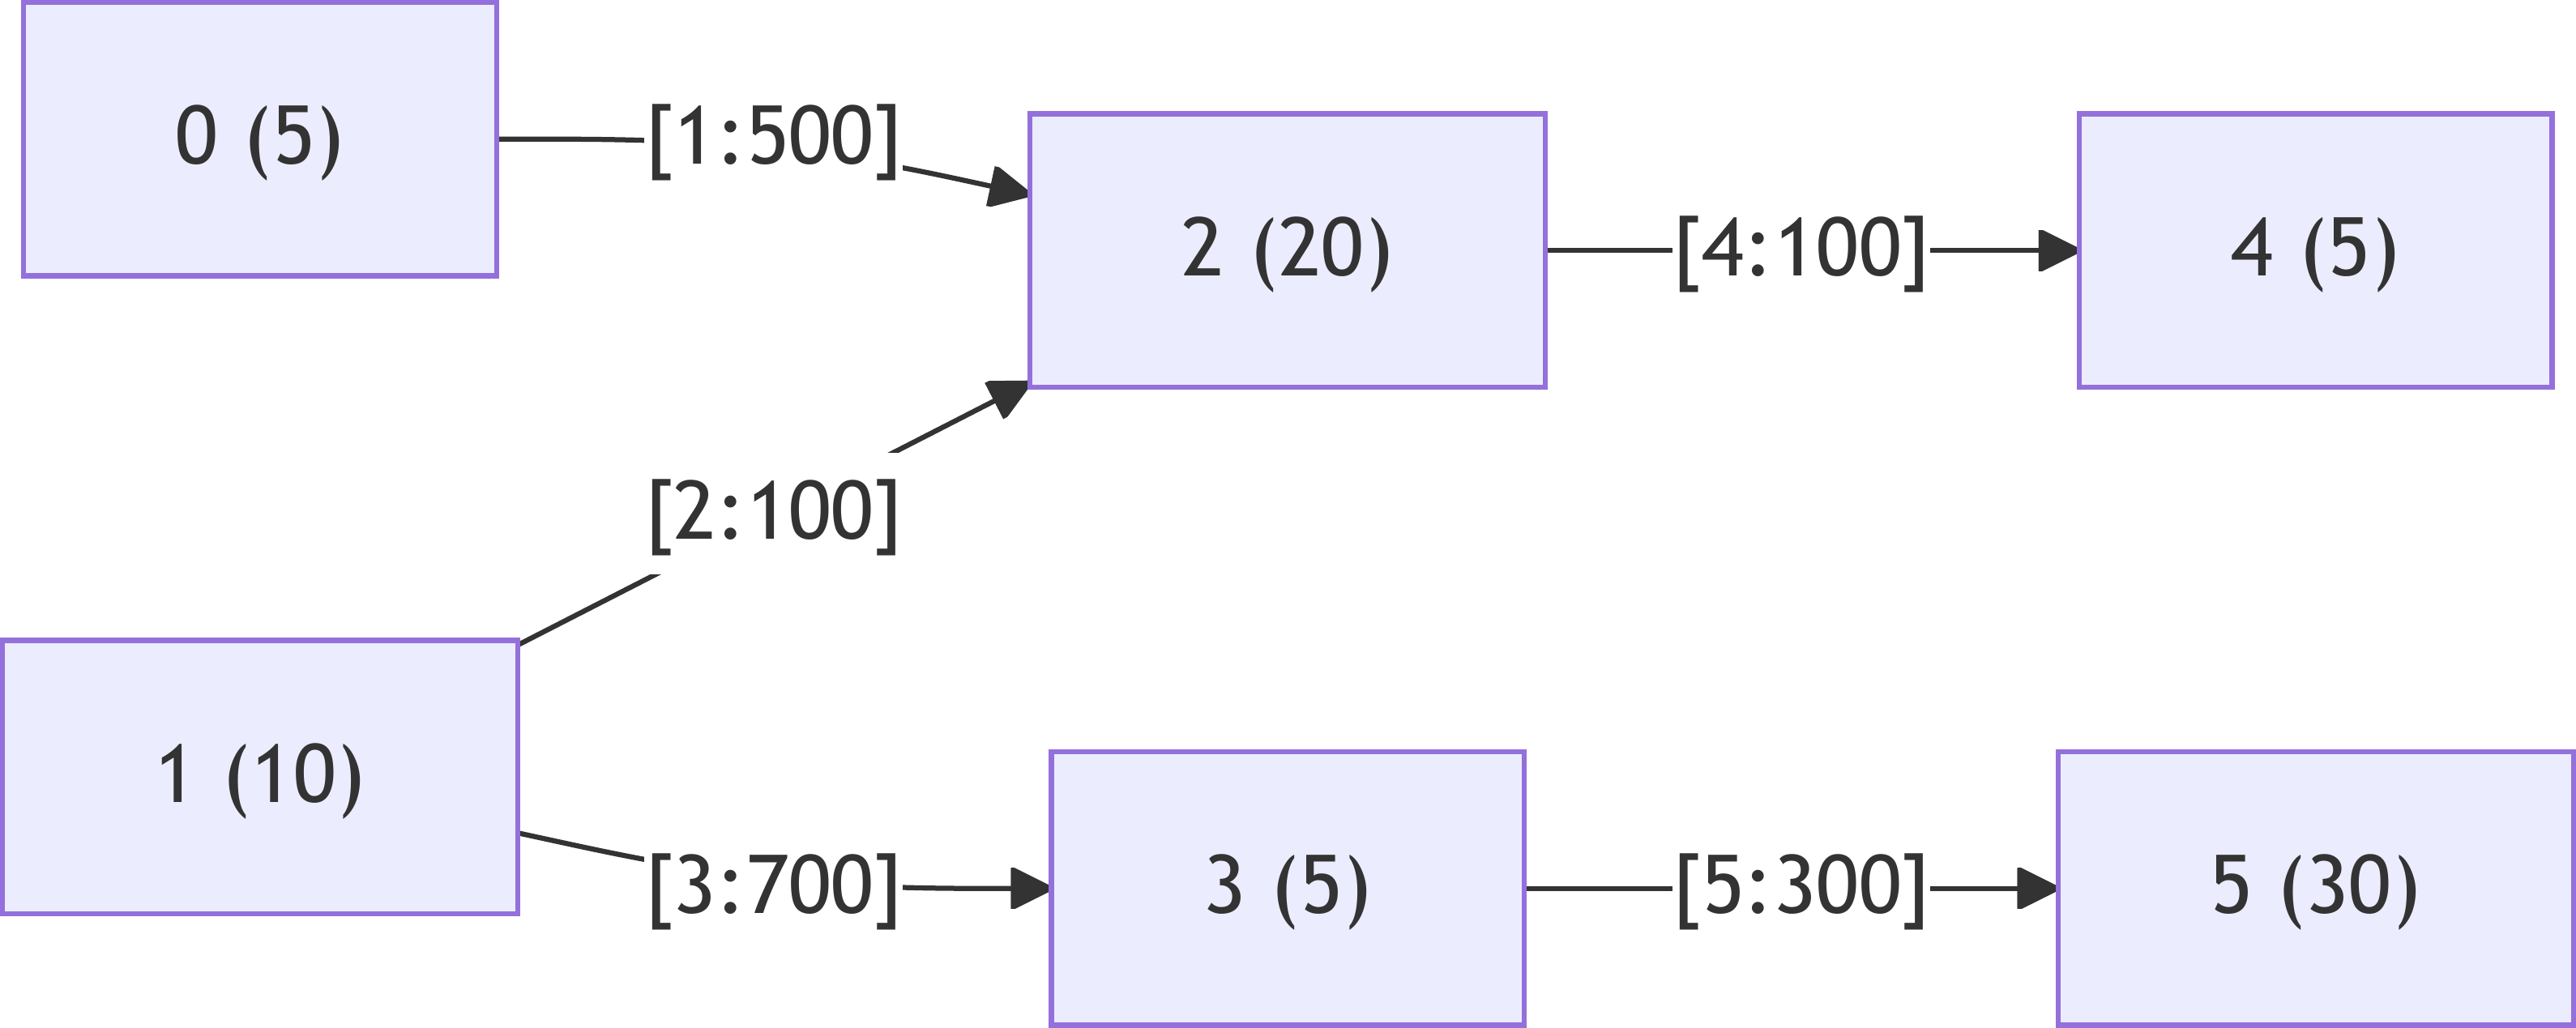
\includegraphics[width=1\textwidth]{pictures/g6-1.png}
	\caption{}
	\label{fig:graph_example}
\end{figure}

\begin{figure}[h]
	\centering
	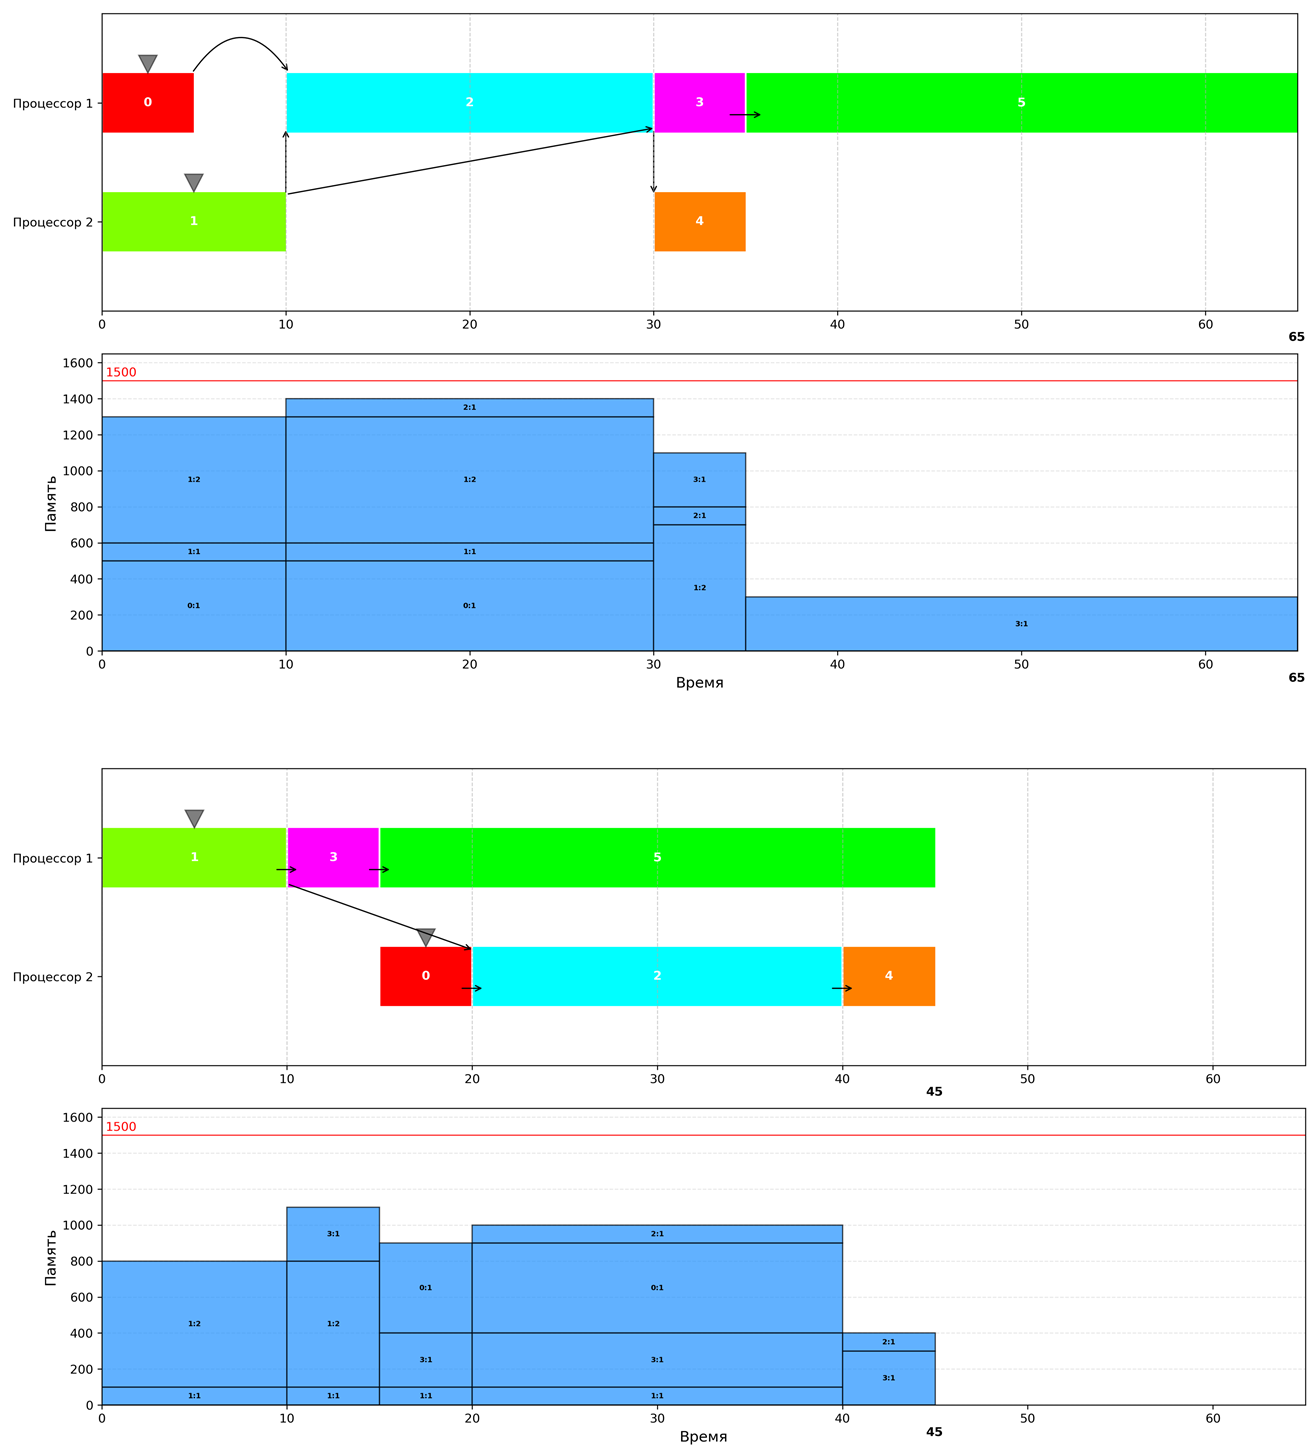
\includegraphics[width=1\textwidth]{pictures/intro2.png}
	\caption{сверху - ЖА с EFT, снизу - ЛП}
	\label{fig:shed_example}
\end{figure}
\section{Цель работы}
\label{sec:1_cel_zadachi} \index{1_cel_zadachi}

\hspace{0.47cm} 

Целью работы является разработка детерминированных алгоритмов построения многопроцессорного расписания с ограничением на объем памяти в целевой системе и минимизацией длительности расписания.

Для достижения цели необходимо:
\begin{enumerate}
    \item разработать жадный алгоритм и эвристики в его составе;
    \item выполнить сведение задачи построения расписания к задаче целочисленного линейного программирования (ЦЛП);
    \item провести экспериментальное исследование жадного алгоритма и подхода на основе ЦЛП по критериям качества решения и длительности его поиска.
\end{enumerate} 
\section{Формальная постановка задачи}
\label{sec:2_problem_statement} \index{2_problem_statement}

\subsection{Модель прикладной программы}
Модель прикладной программы задается ориентированным ациклическим графом потока данных
\[
G = (V, E), \quad |V| = n, \quad |E| = m.
\]
Каждой вершине $v \in V$ соответствует работа, а каждой дуге $(u, v) \in E$ — зависимость по данным между работами $u$ и $v$. Если $(u, v) \in E$, то работа $v$ может начать выполняться только после завершения работы $u$.

Для каждой работы $v \in V$ задана длительность исполнения $d_v > 0$. Кроме того, каждая работа может формировать один или несколько выходных буферов. Обозначим множество буферов, создаваемых работой $v$, через
\[
B(v) = \{b_{v1}, b_{v2}, \dots, b_{vk}\}.
\]
Для каждого буфера $b \in B(v)$ задаются его объем памяти $r_b > 0$ и множество потребителей $C(b) \subseteq V$. Если $u \in C(b)$, то работа $u$ использует результат, содержащийся в буфере $b$.

\subsection{Модель вычислительной системы}
Вычислительная система состоит из $P$ одинаковых процессоров
\[
SP = \{sp_1, sp_2, \dots, sp_P\}.
\]
Каждый процессор в любой момент времени может выполнять не более одной работы. Прерывания работ не допускаются, миграция уже запущенной работы между процессорами невозможна.

Задержки межпроцессорной передачи данных не учитываются. Поэтому момент готовности работы к выполнению определяется завершением всех ее непосредственных предков. Ограничивающими факторами являются зависимости между работами, число доступных процессоров и общий объем памяти $M$, доступный для хранения активных буферов.

\subsection{Модель использования памяти}
Пусть работа $v$ стартует в момент $s_v$ и завершается в момент
\[
f_v = s_v + d_v.
\]
Буфер $b \in B(v)$ выделяется в момент старта работы $v$. В данной модели это означает предварительное резервирование памяти под результат работы: перед запуском работы система должна убедиться, что памяти достаточно для ее выходных буферов, и только после этого работа может быть начата. Освобождение буфера происходит после завершения последней из работ-потребителей его содержимого (в их вершины идут дуги, помеченные этим буфером):
\[
fr_b = \max_{u \in C(b)} f_u.
\]

Обозначим через $J(\tau)$ множество буферов, активных в момент времени $\tau$. Тогда текущее использование памяти равно
\[
\operatorname{mem}(\tau) = \sum_{b \in J(\tau)} r_b.
\]
Пиковое использование памяти на расписании $HP$ определяется как
\[
\operatorname{peak}(HP) = \max_{0 \le \tau \le makespan} (\operatorname{mem}(\tau)).
\]
Расписание считается допустимым по памяти, если выполнено условие
\[
\operatorname{peak}(HP) \le M.
\]

\subsection{Модель расписания}
Расписание $HP$ задает для каждой работы $v \in V$:
\begin{enumerate}
	\item номер процессора $p(v) \in \{1, \dots, P\}$;
	\item момент старта $s_v$;
	\item момент завершения $f_v = s_v + d_v$.
\end{enumerate}
Расписание является корректным, если выполняются следующие ограничения:
\begin{enumerate}
	\item каждая работа назначена ровно одному процессору;
	\item на каждом процессоре интервалы выполнения назначенных ему работ не пересекаются;
	\item для каждой дуги $(u, v) \in E$ выполнено неравенство $f_u \le s_v$;
	\item для всего расписания выполнено ограничение по памяти $\operatorname{peak}(HP) \le M$.
\end{enumerate}

\subsection{Минимизируемая целевая функция}
Минимизируемым критерием является длительность расписания, то есть момент завершения последней работы:
\[
C_{\max}(HP) = \max_{v \in V} f_v.
\]
Требуется найти такое допустимое расписание $HP^*$, что
\[
C_{\max}(HP^*) = \min_{HP \in \mathcal{H}_{\text{adm}}} C_{\max}(HP),
\]
где $\mathcal{H}_{\text{adm}}$ — множество всех корректных расписаний.

Похожие задачи рассматривались в работах~\cite{Wang2010},~\cite{Herrmann2014} и~\cite{Venugopalan2012}, а в работе~\cite{Papp2025} доказывается, что подобная задача является NP-трудной. 
\section{Жадный алгоритм построения многопроцессорного расписания с ограничением на память}
\label{sec:3_greedy_algos} \index{3_greedy_algos}

Жадный алгоритм (ЖА) нужен для быстрого построения корректного расписания на основании некоторой эвристики. При этом не гарантируется оптимальность построенного расписания, но в основе алгоритма лежит локальная стратегия, которая на каждом шаге алгоритма выглядит хорошей с точки зрения минимизации целевой функции. Жадный алгоритм является конструктивным и последовательно достраивает расписание - на каждом шаге алгоритма в соответствии с некоторым критерием выбирается новая работа и добавляется в это расписание. Такой ЖА относится к алгоритмам списочного планирования. Жадные алгоритмы для похожих задач описаны в работах~\cite{Savitsky2023} и~\cite{BalashovKostenko2023}.

\subsection{Формальное описание алгоритма}

Алгоритм работает следующим образом.

\textbf{Шаг 1.} Инициализация. 
\begin{itemize}
	\item Множество ещё не назначенных работ $\mathcal{U} = V$, множество назначенных работ $\mathcal{U'} = \emptyset$.
	\item Множество готовых работ $\mathcal{R} = \{ i \in V \mid \text{у } i \text{ нет предшественников} \}$.
	\item Для каждого процессора $p = 1,\dots,P$ будет храниться набор $Bus_p$ интервалов занятости $[t_{\text{start}}, t_{\text{end}})$, изначально все $Bus_p = \emptyset$.
	\item Для каждого буфера $(i, j)$ вводится интервал активности $Act_{i, j} = [alloc_{i, j}, free_{i, j})$, где $alloc_{i, j}$ будет означать время, когда память была выделена под буфер, а  $free_{i, j}$ -- когда эта память была освобождена. Изначально все $alloc_{i, j} =  free_{i, j} = 0$ (буферы не используются).
\end{itemize}

\textbf{Шаг 2.} Для каждой работы $i \in \mathcal{R}$ и для каждого процессора $p$:
\begin{enumerate}
	\item Найти наиболее раннее время $t$ такое, что:
	\begin{itemize}
		\item процессор $p$ свободен на интервале $[t, t+d_i)$ (нет пересечений с интервалами из $Bus_p$);
		\item для всех предшественников $j$ работы $i$ выполнено $s_j + d_j \le t$;
		\item Для всех моментов $\tau \in [t, t+d_i)$ суммарный объём буферов, у которых еще не все потребители поставлены в расписание, а также буферов $(i', j')$, таких, что $\tau \in Act_{i, j}$, не превышает $(M - sum\_r_i)$, где $sum\_r_i$ -- суммарный объем всех буферов работы $i$.
	\end{itemize}
	\item Если такое $t$ существует, запомнить для пары $(i,p)$ возможное время старта $t_{i,p}$.

	\item Среди всех пар $(i,p)$, для которых найдено допустимое $t_{i,p}$, выбрать одну работу $i^*$ и процессор $p^*$ согласно выбранной эвристике (см. подраздел~\ref{subsec:heuristics}). Если ни одной допустимой пары нет, СТОП (неуспех) -- не удалось построить корректное расписание, либо задача в принципе не имеет решения.

	\item Зафиксировать работу $i^*$ на процессоре $p^*$ со стартом $t = t_{i^*,p^*}$. Обновить расписание: добавить интервал занятости $[t, t+d_{i^*})$ для процессора $p^*$ в набор $Bus_{p*}$, зафиксировать момент старта $s_{i^*}=t$ и завершения $c_{i^*}=t+d_{i^*}$. Обновить состояние памяти: положить $Act_{i, j} = [t, t+d_{i^*})$, а для всех буферов $(i', j')$, таких, что работа $i^*$ использует этот буфер, положить $free_{i',p'} = max(free_{i',p'}, t+d_{i^*})$.
\end{enumerate}

\textbf{Шаг 3.} Удалить $i^*$ из $\mathcal{U}$ и $\mathcal{R}$, добавить $i^*$ в $\mathcal{U'}$. Добавить в $\mathcal{R}$ все работы, у которых работа $i^*$ была последним неназначенным предком. Если $\mathcal{U} \neq \varnothing$, перейти к шагу 2.

\textbf{Шаг 4.} СТОП.\\

В результате получаем полное расписание — для каждой работы определены процессор и время старта.

Блок-схема работы ЖА представлена на рисунке~\ref{fig:gred_sch}.

\begin{center}
	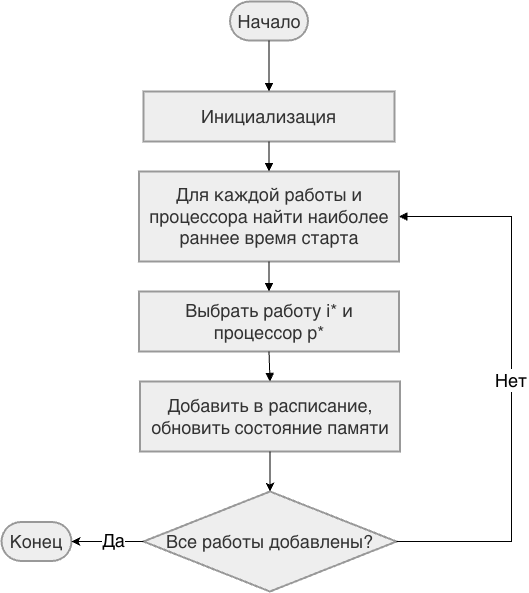
\includegraphics[width=0.63\textwidth]{pictures/gred3.png}
	\captionof{figure}{Блок-схема ЖА}
	\label{fig:gred_sch}
\end{center}

\subsection{Эвристики выбора работы}
\label{subsec:heuristics}

Ключевым элементом жадного алгоритма является правило выбора работы из множества готовых. В данной работе рассматриваются две эвристики: \textbf{EFT} (Earliest Finish Time) и \textbf{STS} (Smallest Time-Space).

\subsubsection*{Эвристика EFT}

Эвристика EFT ориентирована на минимизацию времени завершения работы. После того как для каждой готовой работы $i$ и каждого процессора $p$ определено наиболее раннее допустимое время старта $t_{i,p}$, вычисляется время завершения:
\[
f_{i,p} = t_{i,p} + d_i.
\]
Затем выбирается пара $(i^*, p^*)$, дающая наименьшее $f_{i,p}$. В случае равенства предпочтение отдается работе с наименьшим номером (или процессору с наименьшим номером, если несколько процессоров дают одинаковое время завершения для одной работы). Эта эвристика отличается простотой вычисления, но никак не учитывает использование памяти выбираемой работой.

\subsubsection*{Эвристика STS}

Эвристика STS введена для учёта влияния работы на использование памяти в будущем. Оценка работы складывается из двух компонент.

Первая компонента учитывает собственные буферы работы:
\[
S^{(1)}_i = d_i \cdot \sum_{j=1}^{n_i} r_{ij}.
\]
То есть произведение длительности работы на суммарный объём создаваемых ею буферов.

Вторая компонента учитывает «нагрузку» на память, создаваемую потомками работы. Для каждого буфера $j$ работы $i$ определим множество его потребителей $\mathit{Cons}(i,j) = \{ k \mid (i,k,j) \in E \}$. Пусть $d_{\mathit{total}}(i,j)$ — суммарная длительность всех работ-потребителей этого буфера (каждый потребитель учитывается один раз, даже если он использует несколько буферов). Тогда
\[
S^{(2)}_i = \sum_{j=1}^{n_i} \left( r_{ij} \cdot \sum_{k \in \mathit{Cons}(i,j)} d_k \right).
\]

Общая оценка работы $i$ равна
\[
\phi(i) = S^{(1)}_i + S^{(2)}_i.
\]

Алгоритм выбирает работу с наименьшим значением $\phi(i)$. Если несколько работ имеют одинаковую оценку, то среди них выбирается работа с наименьшим временем завершения (т.е. срабатывает правило EFT). Идея эвристики STS заключается в том, что работа, которая создаёт большие буферы и эти буферы нужны долго выполняющимся потомкам, потребляет память на длительное время, поэтому её выгодно выполнить позже (чтобы не блокировать память). Соответственно, на ранних шагах следует выбирать работы с малым $\phi(i)$.
 
\section{Сведение к задаче целочисленного линейного программирования}
\label{sec:4_reduce_description} \index{4_reduce_description}

\subsection*{Входные данные}
Каждая работа $i$ ($i=1,\dots,n$) характеризуется длительностью $d_i>0$ и набором буферов, которые она создаёт:
\[
V = \bigl\{(i,\; n_i,\; r_{i1}, r_{i2}, \dots, r_{i n_i})\bigr\}_{i=1}^{n},
\]
где $n_i$ — количество буферов работы $i$, а $r_{ij}>0$ — объём памяти, занимаемый $j$-м буфером.  
Дуги графа задают передачу данных:
\[
E = \{(i, k, j)\},\quad j\in[1,n_i],
\]
т.е. дуга $(i,k,j)$ означает, что $j$-й буфер работы $i$ используется работой $k$ (является её входным буфером).  
Все времена $d_i$ целые, допустимый объём памяти равен $M$, число процессоров $P$.

\subsection*{Переменные}

\begin{itemize}
	\item $s_i$ — время старта работы $i$ (целочисленная переменная).
	\item $m_{ij}$ — бинарная переменная, $m_{ij}=1$ если $s_i \le s_j$, иначе $0$ ($i,j=1,\dots,n$).
	\item $p_{ri}$ — бинарная переменная, $p_{ri}=1$ если работа $i$ назначена на процессор $r$ ($r=1,\dots,P$).
	\item $t_{ij}$ — бинарная переменная, $t_{ij}=1$ если работы $i$ и $j$ выполняются на одном процессоре.
	\item $l$ — целочисленная переменная, общая длительность расписания (makespan).
	\item Для каждого буфера $(i,j)$ ($j=1,\dots,n_i$) вводятся целочисленные переменные:
	\[
	\text{start}_{ij},\quad \text{max\_end}_{ij}.
	\]
	$\text{start}_{ij}$ совпадает со стартом работы $i$, а $\text{max\_end}_{ij}$ — максимальное время завершения среди всех потребителей этого буфера.
	\item Для каждой пары буферов $(i,j)$ и $(p,q)$ вводятся бинарные переменные:
	\[
	z_{ij}^{pq},\; zz_{ij}^{pq},\; a_{ij}^{pq},\; aa_{ij}^{pq}.
	\]
	Они служат для моделирования пересечений интервалов активности буферов.
\end{itemize}

\subsection*{Вспомогательная константа}

\[
D = \sum_{i=1}^{n} d_i,
\]
которая заведомо больше любого возможного makespan.

\subsection*{Ограничения, связывающие $m_{ij}$ и $s_i$}

Для всех $i,j$:
\begin{align}
	m_{ii} &= 1, \label{eq:m_diag}\\
	D\,m_{ij} - s_j + s_i &\ge 0, \label{eq:m_ge}\\
	s_j - s_i - D\,m_{ij} &\ge 1 - D. \label{eq:m_le}
\end{align}
Эти условия эквивалентны: $m_{ij}=1 \Leftrightarrow s_i \le s_j$.

\subsection*{Назначение на процессоры}

Для всех $i$ и $r$:
\begin{align}
	\sum_{r=1}^{P} p_{ri} &= 1, \label{eq:p_sum}\\
	p_{ri} &\in \{0,1\}. \nonumber
\end{align}

\subsection*{Переменные $t_{ij}$ (один процессор)}

Для всех $i,j,k$ ($i\neq j$) и всех $r$:
\begin{align}
	t_{ij} &\ge p_{ri} + p_{rj} - 1, \label{eq:t_ge}\\
	t_{ij} &\le p_{ri} - p_{rj} + 1, \label{eq:t_le}\\
	t_{ij} &\in \{0,1\}. \nonumber
\end{align}
При этом $t_{ij}=1$ тогда и только тогда, когда $p_{ri}=p_{rj}=1$ для некоторого $r$.

\subsection*{Зависимости по графу}

Для каждой дуги $(i,k,j)\in E$ (т.е. $j$-й буфер работы $i$ потребляется работой $k$):
\begin{align}
	s_k \ge s_i + d_i. \label{eq:prec}
\end{align}

\subsection*{Определение $\text{start}_{ij}$ и $\text{max\_end}_{ij}$}

Для каждого буфера $(i,j)$:
\begin{align}
	\text{start}_{ij} &= s_i, \label{eq:start_def}\\
	\text{max\_end}_{ij} &\ge s_k + d_k \quad \text{для всех } k \text{ таких, что } (i,k,j)\in E. \label{eq:max_end_def}
\end{align}
Таким образом, $\text{max\_end}_{ij}$ — максимум моментов завершения всех потребителей буфера.

\subsection*{Взаимное исключение на одном процессоре}

Для всех $i\neq j$:
\begin{align}
	s_i - s_j + D\,m_{ij} - D\,t_{ij} &\ge -D + d_j, \label{eq:no_conflict1}\\
	s_j - s_i - D\,m_{ij} - D\,t_{ij} &\ge -2D + d_i. \label{eq:no_conflict2}
\end{align}
Если $t_{ij}=1$ (работы на одном процессоре), то эти ограничения вынуждают $s_j \ge s_i + d_i$ при $m_{ij}=1$ и $s_i \ge s_j + d_j$ при $m_{ij}=0$. При $t_{ij}=0$ ограничения выполняются автоматически.

\subsection*{Учёт пересечений буферов (для ограничения памяти)}

Для каждой пары буферов $(i,j)$ и $(p,q)$ введём вспомогательные бинарные переменные $z_{ij}^{pq}$, $zz_{ij}^{pq}$, $a_{ij}^{pq}$, $aa_{ij}^{pq}$, связанные следующими линейными ограничениями:
\begin{align}
	\text{start}_{pq} - \text{start}_{ij} - (D+1)\,z_{ij}^{pq} &\ge -D, \label{eq:z_start}\\
	(D+1)\,a_{ij}^{pq} + (D+1)\,z_{ij}^{pq} + \text{start}_{ij} - \text{max\_end}_{pq} &\ge 0, \label{eq:a_start}\\
	\text{start}_{pq} - \text{max\_end}_{ij} - (D+1)\,zz_{ij}^{pq} &\ge -D, \label{eq:zz_end}\\
	(D+1)\,aa_{ij}^{pq} + (D+1)\,zz_{ij}^{pq} + \text{max\_end}_{ij} - \text{max\_end}_{pq} &\ge 0. \label{eq:aa_end}
\end{align}
Переменные $a_{ij}^{pq}$ и $aa_{ij}^{pq}$ интерпретируются следующим образом:
\begin{itemize}
	\item $a_{ij}^{pq}=1$, если буфер $(p,q)$ активен в момент старта буфера $(i,j)$ (т.е. $\text{start}_{ij}$ лежит внутри интервала активности $(p,q)$);
	\item $aa_{ij}^{pq}=1$, если буфер $(p,q)$ активен в момент завершения буфера $(i,j)$ (т.е. $\text{max\_end}_{ij}$ лежит внутри интервала активности $(p,q)$).
\end{itemize}
Интервал активности буфера $(p,q)$ — это $[\text{start}_{pq},\; \text{max\_end}_{pq})$.

\subsection*{Ограничение на суммарную память}

Для каждого буфера $(i,j)$ суммарный объём памяти, занятый в момент $\text{start}_{ij}$ (соответственно $\text{max\_end}_{ij}$), не должен превышать $M$:
\begin{align}
	\sum_{(p,q)} r_{pq}\, a_{ij}^{pq} &\le M, \label{eq:mem_start}\\
	\sum_{(p,q)} r_{pq}\, aa_{ij}^{pq} &\le M, \label{eq:mem_end}
\end{align}
где сумма берётся по всем буферам, присутствующим в графе. Благодаря определению $a_{ij}^{pq}$ и $aa_{ij}^{pq}$, эти ограничения гарантируют, что пиковое потребление памяти в любой момент (все точки вида $\text{start}_{ij}$ или $\text{max\_end}_{ij}$) не превышает $M$.

\subsection*{Целевая функция}

Минимизируем общую длительность расписания:
\begin{align}
	\min \; l,\\
	l \ge s_i + d_i \quad \forall i. \label{eq:l_bound}
\end{align}

\subsection*{Итоговая задача}

\[
\begin{array}{ll}
	\text{Минимизировать} & l \\
	\text{при ограничениях} & (\ref{eq:m_diag})—(\ref{eq:m_le}),\; (\ref{eq:p_sum}),\; (\ref{eq:t_ge})—(\ref{eq:t_le}),\; (\ref{eq:prec}),\; (\ref{eq:start_def}),\; (\ref{eq:max_end_def}),\\
	& (\ref{eq:no_conflict1})—(\ref{eq:no_conflict2}),\; (\ref{eq:z_start})—(\ref{eq:aa_end}),\; (\ref{eq:mem_start})—(\ref{eq:mem_end}),\; (\ref{eq:l_bound}),\\
	& \text{переменные } s_i,\text{start}_{ij},\text{max\_end}_{ij},l\in\mathbb{Z}_{\ge0},\; 
	m_{ij},p_{ri},t_{ij},z_{ij}^{pq},zz_{ij}^{pq},a_{ij}^{pq},aa_{ij}^{pq}\in\{0,1\}.
\end{array}
\]

\subsection*{Число переменных и ограничений}

Пусть $n$ — число работ, $n_i$ — число буферов работы $i$, $B=\sum_i n_i$ — общее число буферов, $P$ — число процессоров. Тогда:
\begin{itemize}
	\item $m_{ij}$: $n^2$ бинарных.
	\item $s_i$: $n$ целых.
	\item $p_{ri}$: $P n$ бинарных.
	\item $t_{ij}$: $n^2$ бинарных.
	\item $\text{start}_{ij},\text{max\_end}_{ij}$: $2B$ целых.
	\item $z_{ij}^{pq}, zz_{ij}^{pq}, a_{ij}^{pq}, aa_{ij}^{pq}$: $4B^2$ бинарных.
	\item $l$: одна целая.
\end{itemize}
Количество ограничений составляет $O(n^2 + P n + |E| + B^2)$. 
\section{Экспериментальное исследование}
\label{sec:5_experiments} \index{5_experiments}

\subsection{Предмет и цели исследования}
\label{subsec:goals}

Предметом исследования являются предложенные подходы к решению задачи: жадный алгоритм с эвристиками EFT и STS; подход на основе ЦЛП. Целями исследования является сравнительный анализ подходов по следующим критериям:

- качество получаемого решения (т.е. значение целевой функции на расписании);

- масштабируемость по времени поиска решения при увеличении размерности входных данных. 

\subsection{Классы графов работ}
\label{subsec:graph_classes}

Используются три класса ориентированных ациклических графов:

\subsubsection{Слоистые графы}
Слоистые графы (рис.~\ref{fig:layered}) характерны для многоэтапных вычислений (цифровая обработка сигналов, научные расчёты).  
Вершины разбиты на последовательные слои, рёбра в основном соединяют вершины соседних слоёв, но допускаются «перескоки» через несколько слоёв.

\begin{figure}[h]
	\centering
	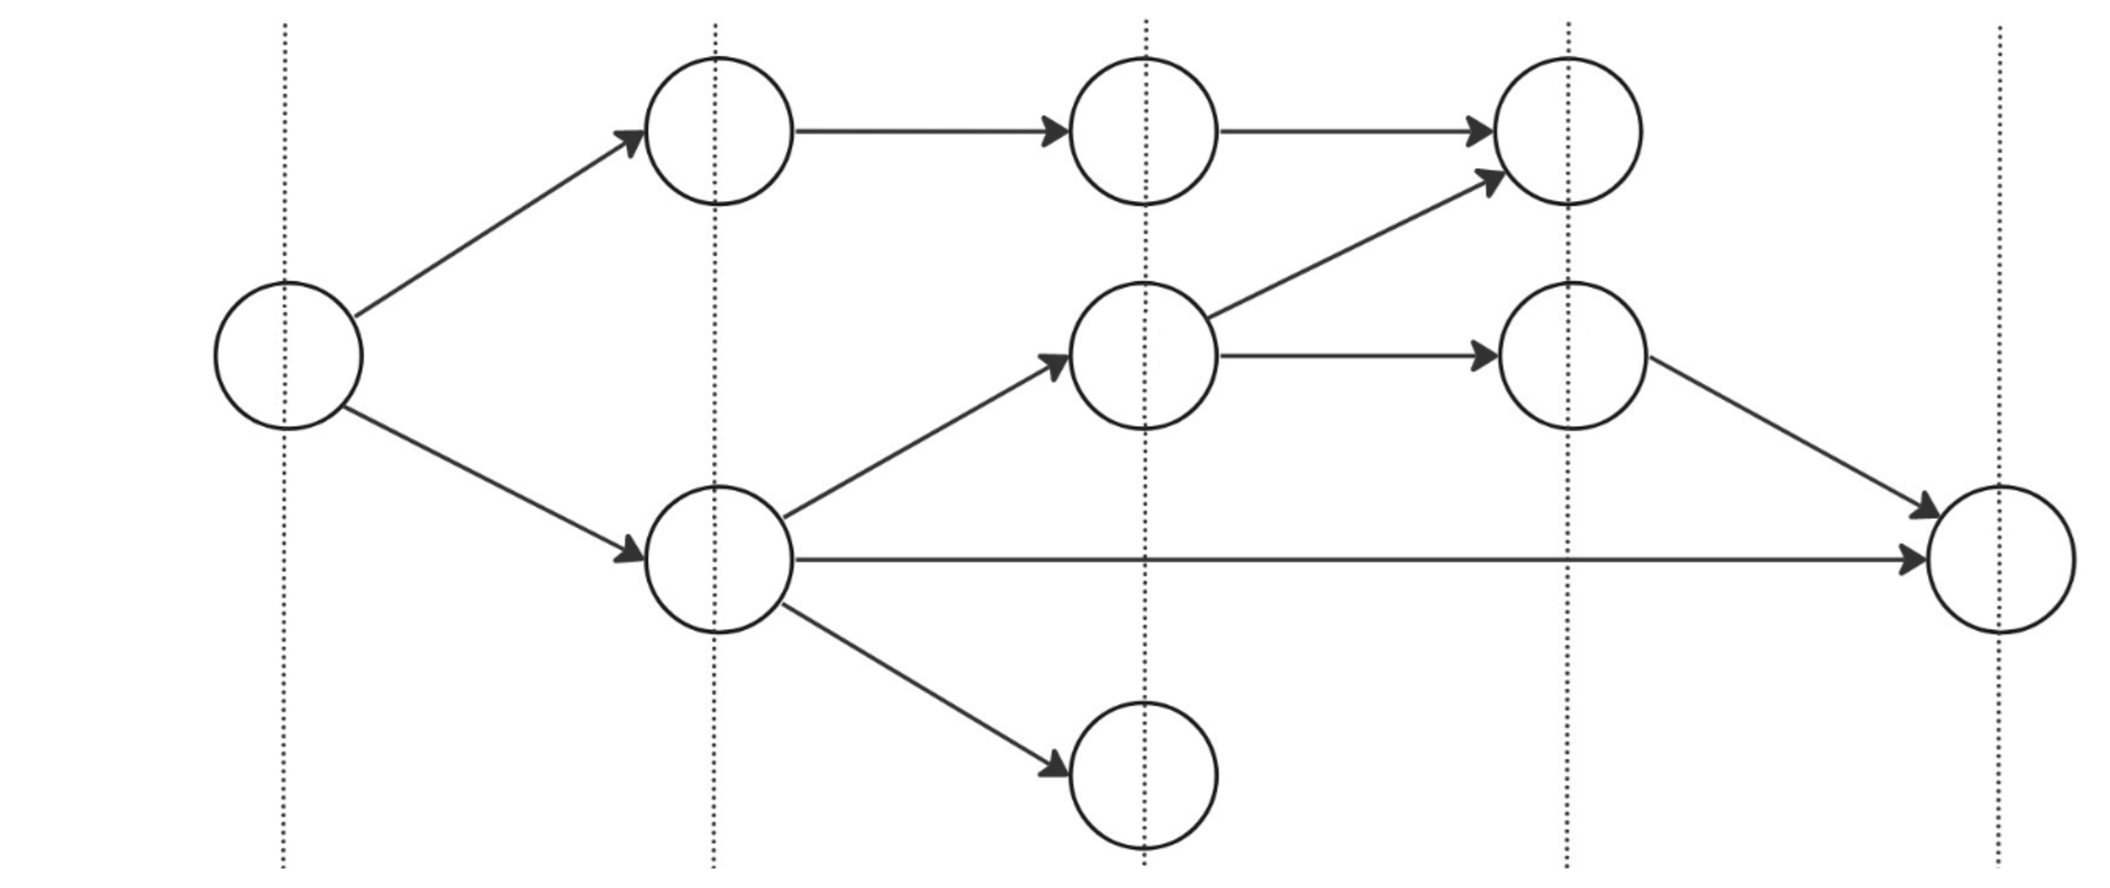
\includegraphics[width=0.5\textwidth]{pictures/layered_graph_scheme.eps}
	\caption{Пример слоистого графа}
	\label{fig:layered}
\end{figure}

\subsubsection{Случайные графы}
Случайные графы (рис.~\ref{fig:random}) генерируются с ограничениями: у каждой вершины не более двух предков и не более шести потомков. Такие графы встречаются, например, при реализации LU- и QR-разложений.

\begin{figure}[h]
	\centering
	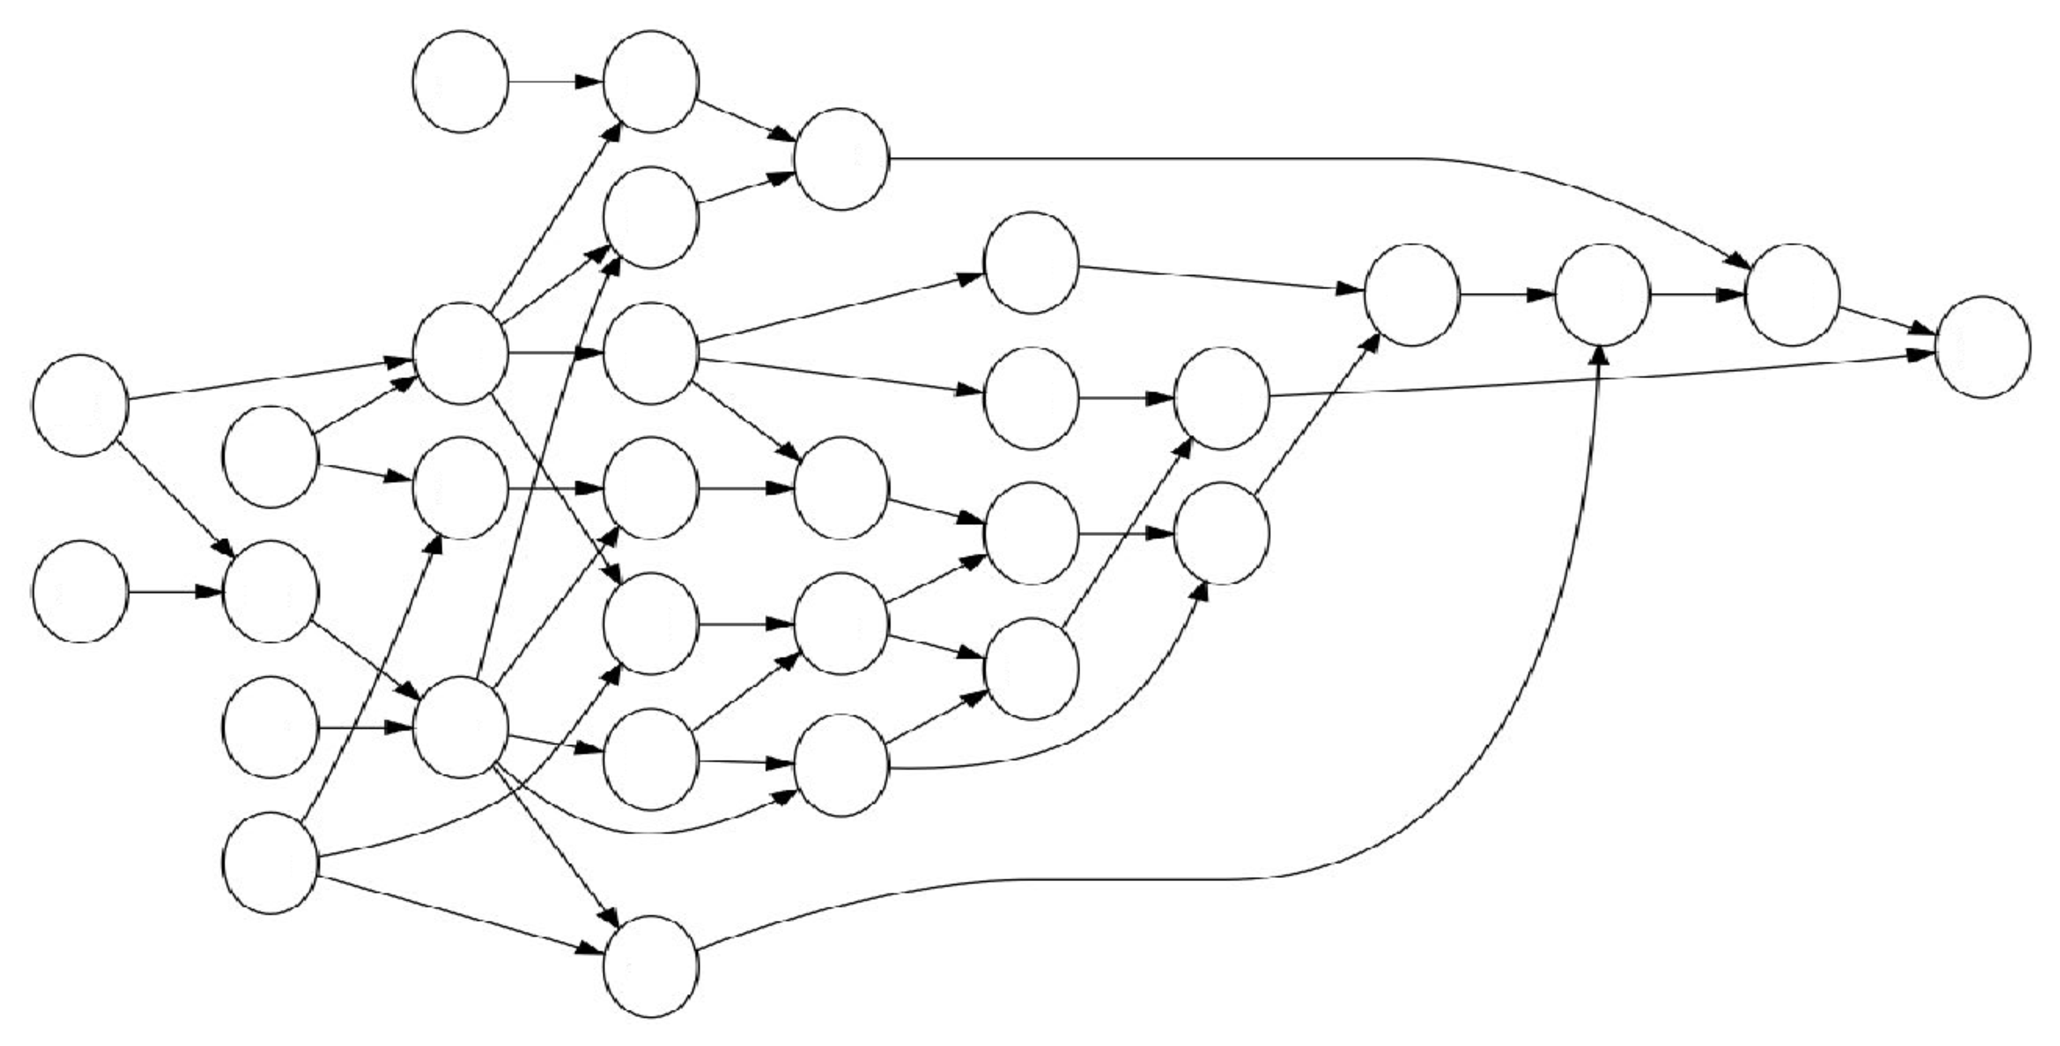
\includegraphics[width=0.5\textwidth]{pictures/random_graph_scheme.eps}
	\caption{Пример случайного графа}
	\label{fig:random}
\end{figure}

\subsubsection{Треугольные графы}
Треугольные графы (рис.~\ref{fig:triangular}) — частный случай слоистых графов, моделирующий метод Гаусса–Жордана.  
Они обладают регулярной структурой: каждый слой содержит на одну вершину меньше предыдущего, рёбра соединяют только соседние слои. Используются только для больших размеров задач.

\begin{figure}[h]
	\centering
	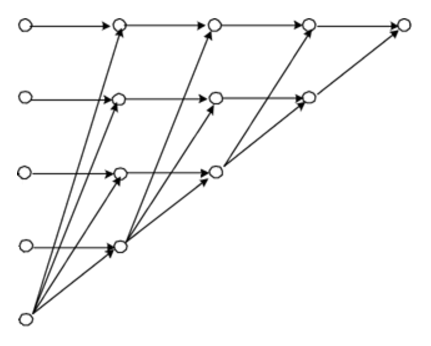
\includegraphics[width=0.5\textwidth]{pictures/triang_graph_scheme.eps}
	\caption{Пример треугольного графа}
	\label{fig:triangular}
\end{figure}

\subsection{Наборы входных данных}
\label{subsec:datasets}

Для каждого из двух исследований (качество и масштабируемость) используются отдельные наборы графов, различающиеся размерностью.  
Все графы имеют следующие общие параметры:

\begin{itemize}
	\item Длительность работы $d_i$ — целое число, равномерно распределённое в диапазоне $[10, 100]$.
	\item Вес каждого буфера — целое число, равномерно распределённое в диапазоне $[1, 100]$.
	\item Для каждой работы используются два варианта формирования буферов:
	\begin{enumerate}
		\item \textbf{Один буфер}: все исходящие рёбра объединены в один буфер указанного веса.
		\item \textbf{Корневое равномерное распределение}: количество буферов равно $\lceil\sqrt{\text{outdeg}}\rceil$, рёбра распределяются по буферам максимально равномерно.
	\end{enumerate}
\end{itemize}

\subsubsection{Малые графы}

\begin{itemize}
	\item \textbf{Слоистые графы}: все размеры $n = 10, 11, \dots, 21$ (по одному графу на размер).
	\item \textbf{Случайные графы}: все размеры $n = 10, 11, \dots, 21$ (по одному графу на размер).
\end{itemize}

\subsubsection{Большие графы}

\begin{itemize}
	\item \textbf{Слоистые графы}: по одному графу для каждого размера $n \in \{55, 210, 496, 990\}$.
	\item \textbf{Случайные графы}: по одному графу для каждого размера $n \in \{55, 210, 496, 990\}$.
	\item \textbf{Треугольные графы}:
	\begin{itemize}
		\item Для оценки качества: по одному графу для каждого размера $n \in \{55, 210, 496, 990\}$
		\item Для оценки масштабируемости: расширенная сетка размеров - по одному графу для каждого размера $n \in \{55, 105, 153, 210, 300, 496, 741, 990\}$ 
	\end{itemize}
\end{itemize}

\subsubsection{Сетка параметров $(P, M)$}

Для каждого графа предварительно определяются:
\begin{itemize}
	\item $P_{\max}$ — максимальное число процессоров, которое может эффективно использовать жадный алгоритм на данном графе при заведомо избыточной памяти.
	\item $M_{\max}$ — максимальная пиковая память, возникающая при выполнении расписания с заведомо избыточным числом процессоров.
\end{itemize}

\noindent \textbf{Число процессоров $P$:}
\begin{itemize}
	\item Если $P_{\max} \ge 50$, то $P \in \{4,\; \lfloor(4+P_{\max})/2\rfloor,\; P_{\max}\}$.
	\item Если $P_{\max} < 50$, то $P \in \{2,\; \lfloor(2+P_{\max})/2\rfloor,\; P_{\max}\}$.
\end{itemize}

\noindent \textbf{Лимит памяти $M$:}
\begin{itemize}
	\item Для малых графов ($n \le 21$): $M_{\min}=1$, поиск ведётся с шагом $1$ до первого допустимого расписания.
	\item Для больших графов ($n \ge 55$): $M_{\min} = \lfloor M_{\max}/10\rfloor$, шаг поиска $\Delta M = \lfloor M_{\max}/100\rfloor$.
	\item В обоих случаях используются три уровня: $M \in \{M_{\min},\; \lfloor(M_{\min}+M_{\max})/2\rfloor,\; M_{\max}\}$.
\end{itemize}

Таким образом, для каждого исходного графа формируется 9 вариантов входных данных ($3\times3$ комбинации $P$ и $M$), на которых проводятся запуски.

\subsection{Результаты экспериментов}

Эксперименты проводились на компьютере со следующими характеристиками:
\begin{itemize}
	\item ЦП: Apple M1
	\item Количество ядер: 8;
	\item Объём ОЗУ: 16 Гбайт;
	\item ОС: macOS Sonoma 14.5.
\end{itemize}

\paragraph{Выбор решателя и схема параллельного запуска}

В качестве решателя задач целочисленного линейного программирования используется SCIP. Выбор обоснован в работе А.К.~Сенюшкиной~\cite{senyushkina2025}, где проведено сравнительное исследование производительности свободно доступных решателей (GLPK, CBC, SCIP) на графах рассматриваемых классов; SCIP показал наилучшие результаты по времени поиска оптимального решения.

Из-за значительной зависимости времени работы решателя от упорядочения переменных и ограничений, а также от добавления транзитивных рёбер (см.~\cite{balashov_senyushkina2024}), применяется метод «параллельного запуска с остановкой по первому успеху». Для каждого входного графа формируются 8 вариантов \texttt{.lp}-файлов, соответствующих комбинациям:
\begin{itemize}
	\item 4 упорядочения вершин и рёбер: \texttt{default}, \texttt{up\_right}, \texttt{down\_left}, \texttt{tiers};
	\item 2 варианта графа: с добавленными транзитивными ограничениями (флаг \texttt{-tr}) и без них.
\end{itemize}
(Упорядочение \texttt{reverse\_tiers} не используется из-за ограниченности числа доступных процессорных ядер.)

Затем скрипт \texttt{run\_scip2.sh} одновременно запускает 8 экземпляров SCIP по одному на каждый вариант. Как только хотя бы один экземпляр завершается с нахождением оптимального решения (статус \texttt{optimal solution found}), все остальные процессы принудительно завершаются. Это позволяет избежать неоправданного ожидания на «медленных» упорядочениях и эффективно использовать доступные вычислительные ресурсы. Лимит времени на каждый экземпляр задаётся в файле \texttt{only\_time.set} (в экспериментах использовалось 3600 секунд).

\subsubsection{Малые графы}

\subsubsection*{Исследование масштабируемости}

\begin{center}
	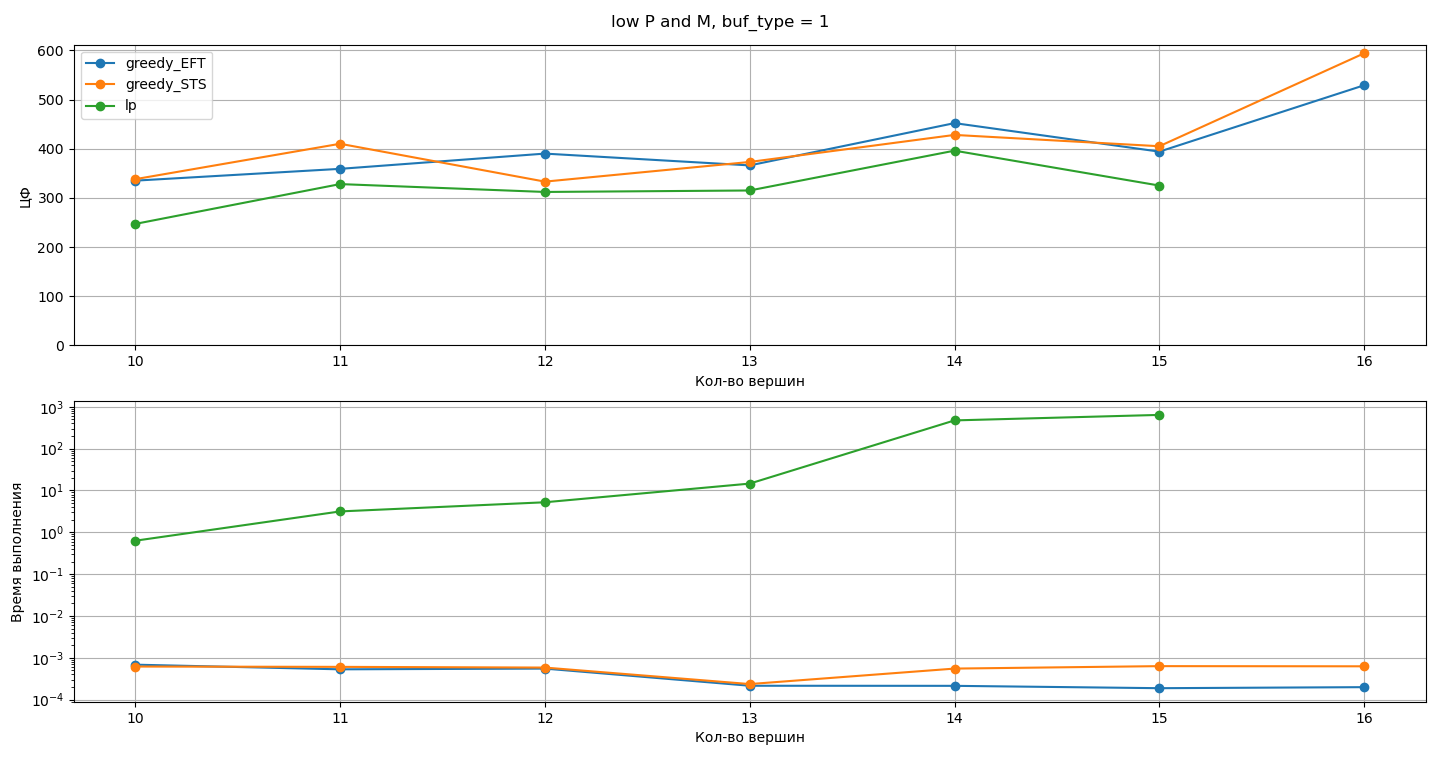
\includegraphics[width=1\textwidth]{pictures/lowPM_1_S.png}
	\captionof{figure}{описание 1}
	\label{fig:scal1}
\end{center}

\begin{center}
	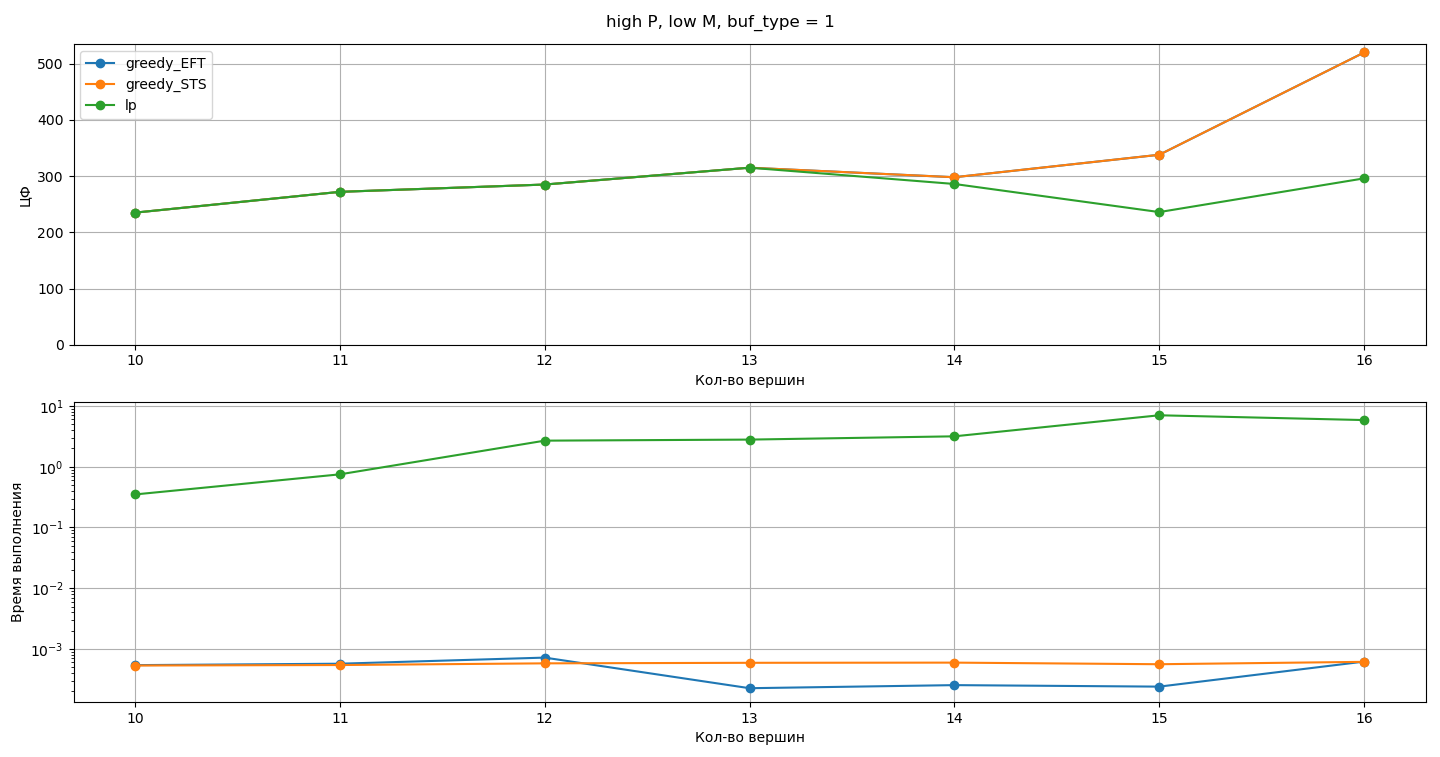
\includegraphics[width=1\textwidth]{pictures/highPlowM_1_S.png}
	\captionof{figure}{описание 2}
	\label{fig:scal2}
\end{center}

\begin{center}
	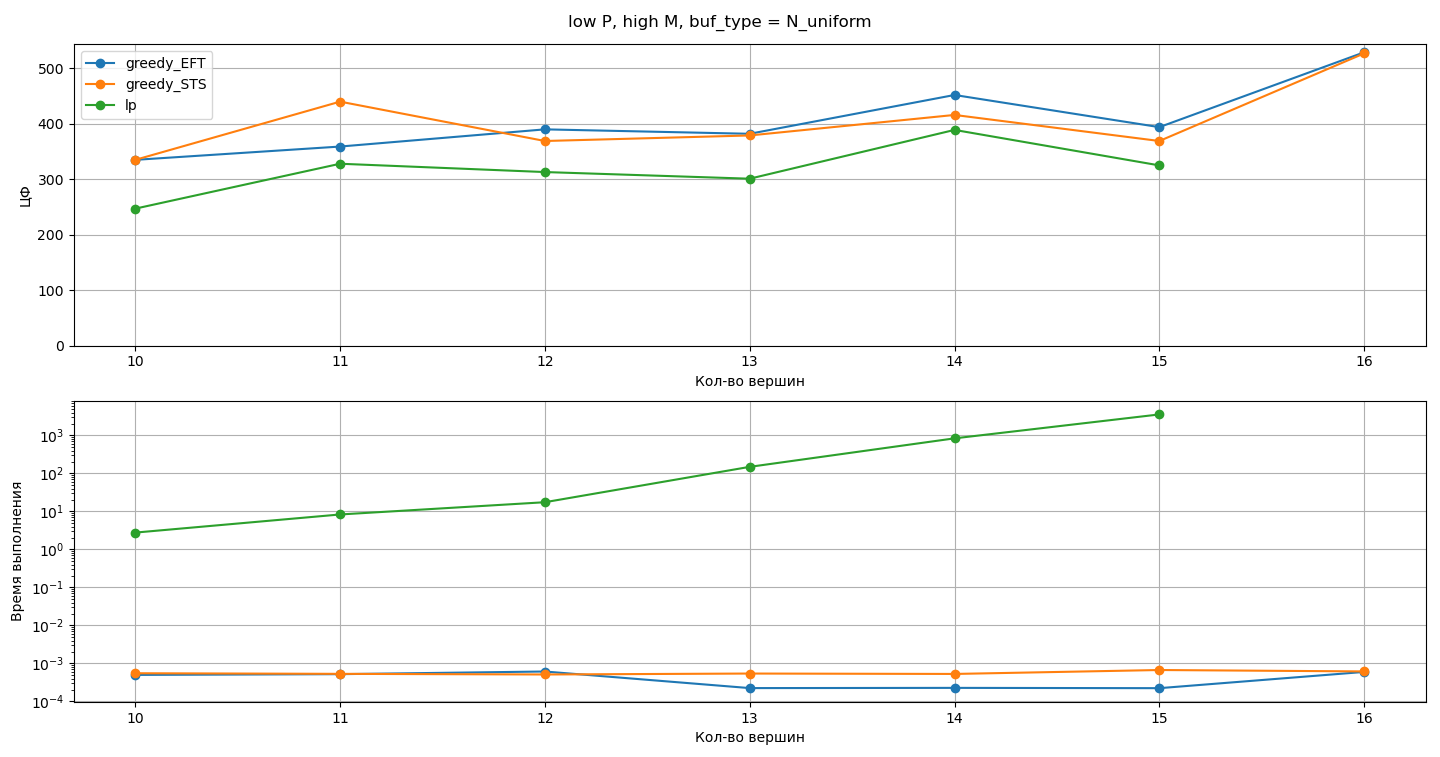
\includegraphics[width=1\textwidth]{pictures/lowPhighM_N_S.png}
	\captionof{figure}{описание 3}
	\label{fig:scal3}
\end{center}

\subsubsection*{Исследование качества решения}

\begin{center}
	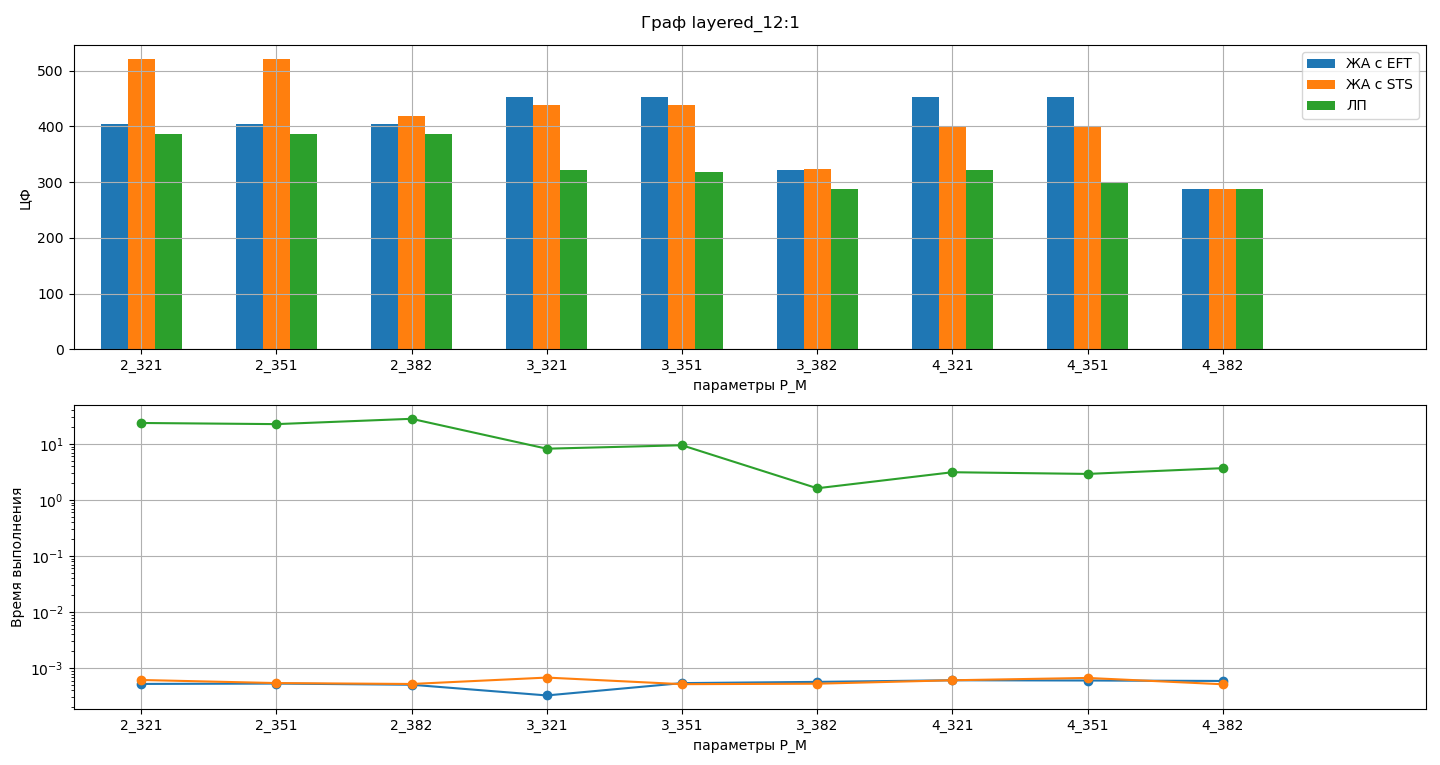
\includegraphics[width=1\textwidth]{pictures/layered_12_1.png}
	\captionof{figure}{описание 4}
	\label{fig:scal3}
\end{center}

\begin{center}
	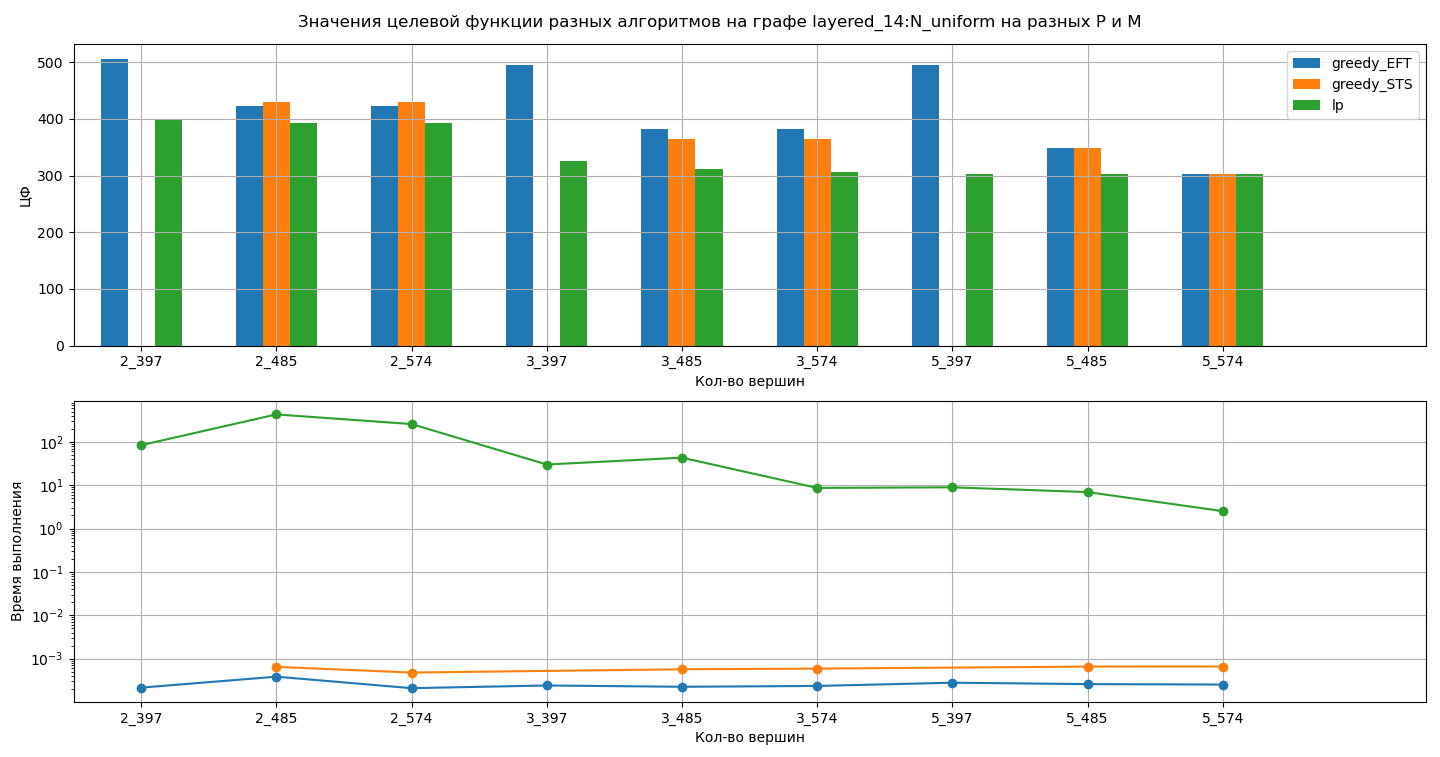
\includegraphics[width=1\textwidth]{pictures/layered_14_N.png}
	\captionof{figure}{описание 5}
	\label{fig:scal3}
\end{center}

\begin{center}
	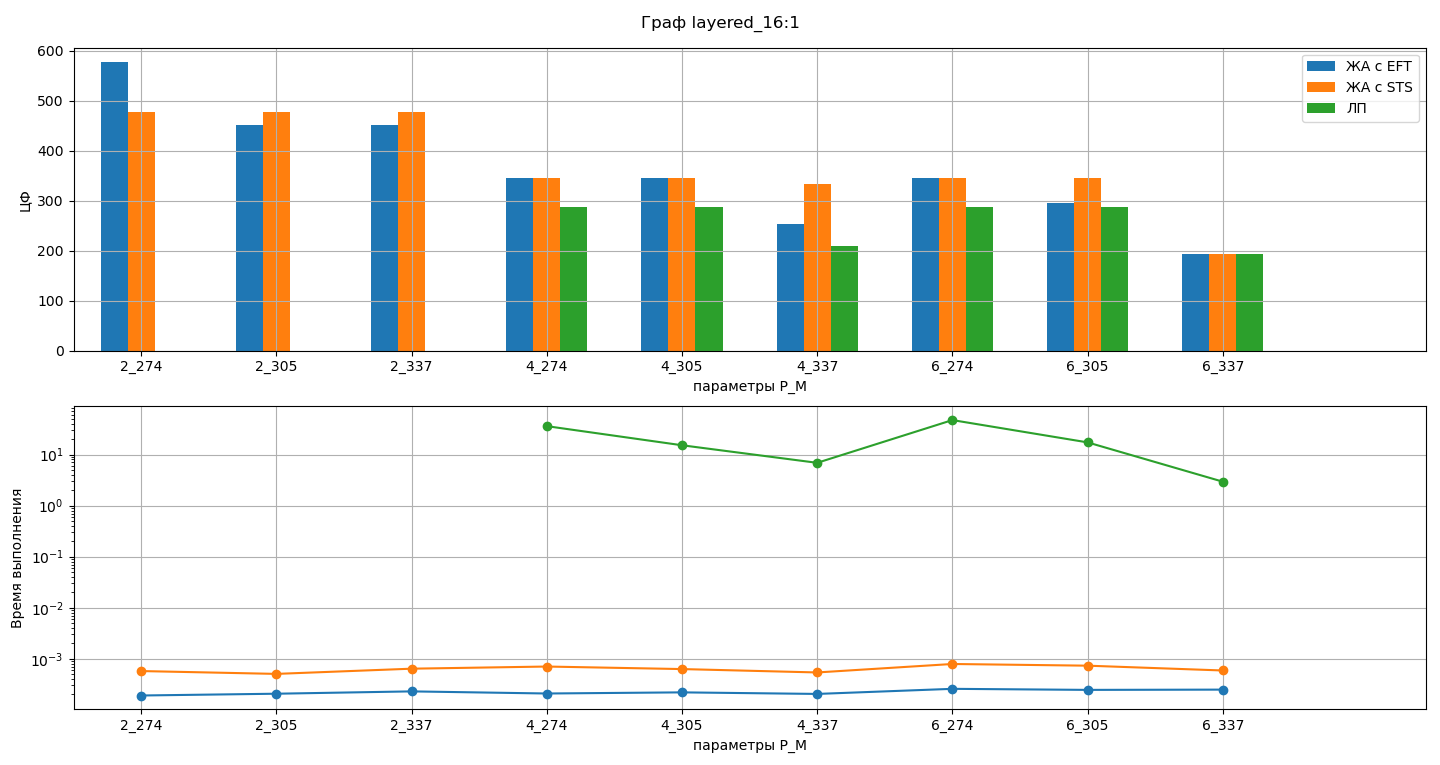
\includegraphics[width=1\textwidth]{pictures/layered_16_1.png}
	\captionof{figure}{описание 6}
	\label{fig:scal3}
\end{center}

\begin{center}
	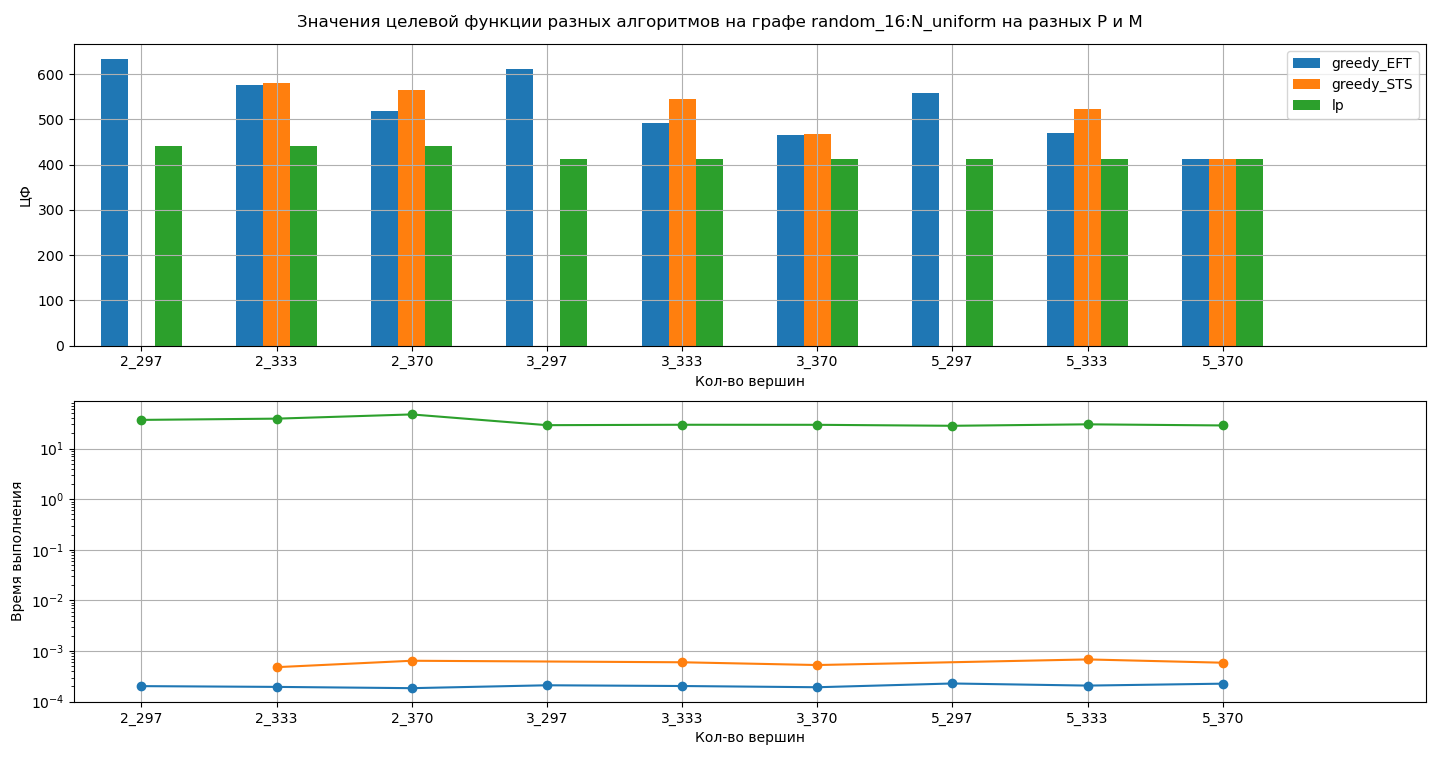
\includegraphics[width=1\textwidth]{pictures/random_16_N.png}
	\captionof{figure}{описание 7}
	\label{fig:scal3}
\end{center} 
\section{Описание программной реализации}
\label{sec:6_programs} \index{6_programs}

Все файлы доступны в репозитории\footnote{URL: \url{https://github.com/Grenkas321/Coursework}} в ветке Max\_multiprocessing. Реализация ЖА содержится в папке algorithms, файлы для ЛП -- в папке LP, средства визуализации -- в папке visualisation. Общий объем программ -- около 221 Кб, около 5000 строк кода.

\subsection{Реализация жадного алгоритма}\label{sec:real_greedy}

Программная реализация жадного алгоритма с двумя эвристиками выполнена на языке C++ (стандарт C++17). В основе реализации лежит модульная архитектура, позволяющая легко добавлять новые эвристики и конфигурировать параметры (число процессоров, лимит памяти). Основные классы и их взаимосвязи показаны на диаграмме (рис.~\ref{fig:greedy_class_diagram}).

\begin{figure}[h]
	\centering
	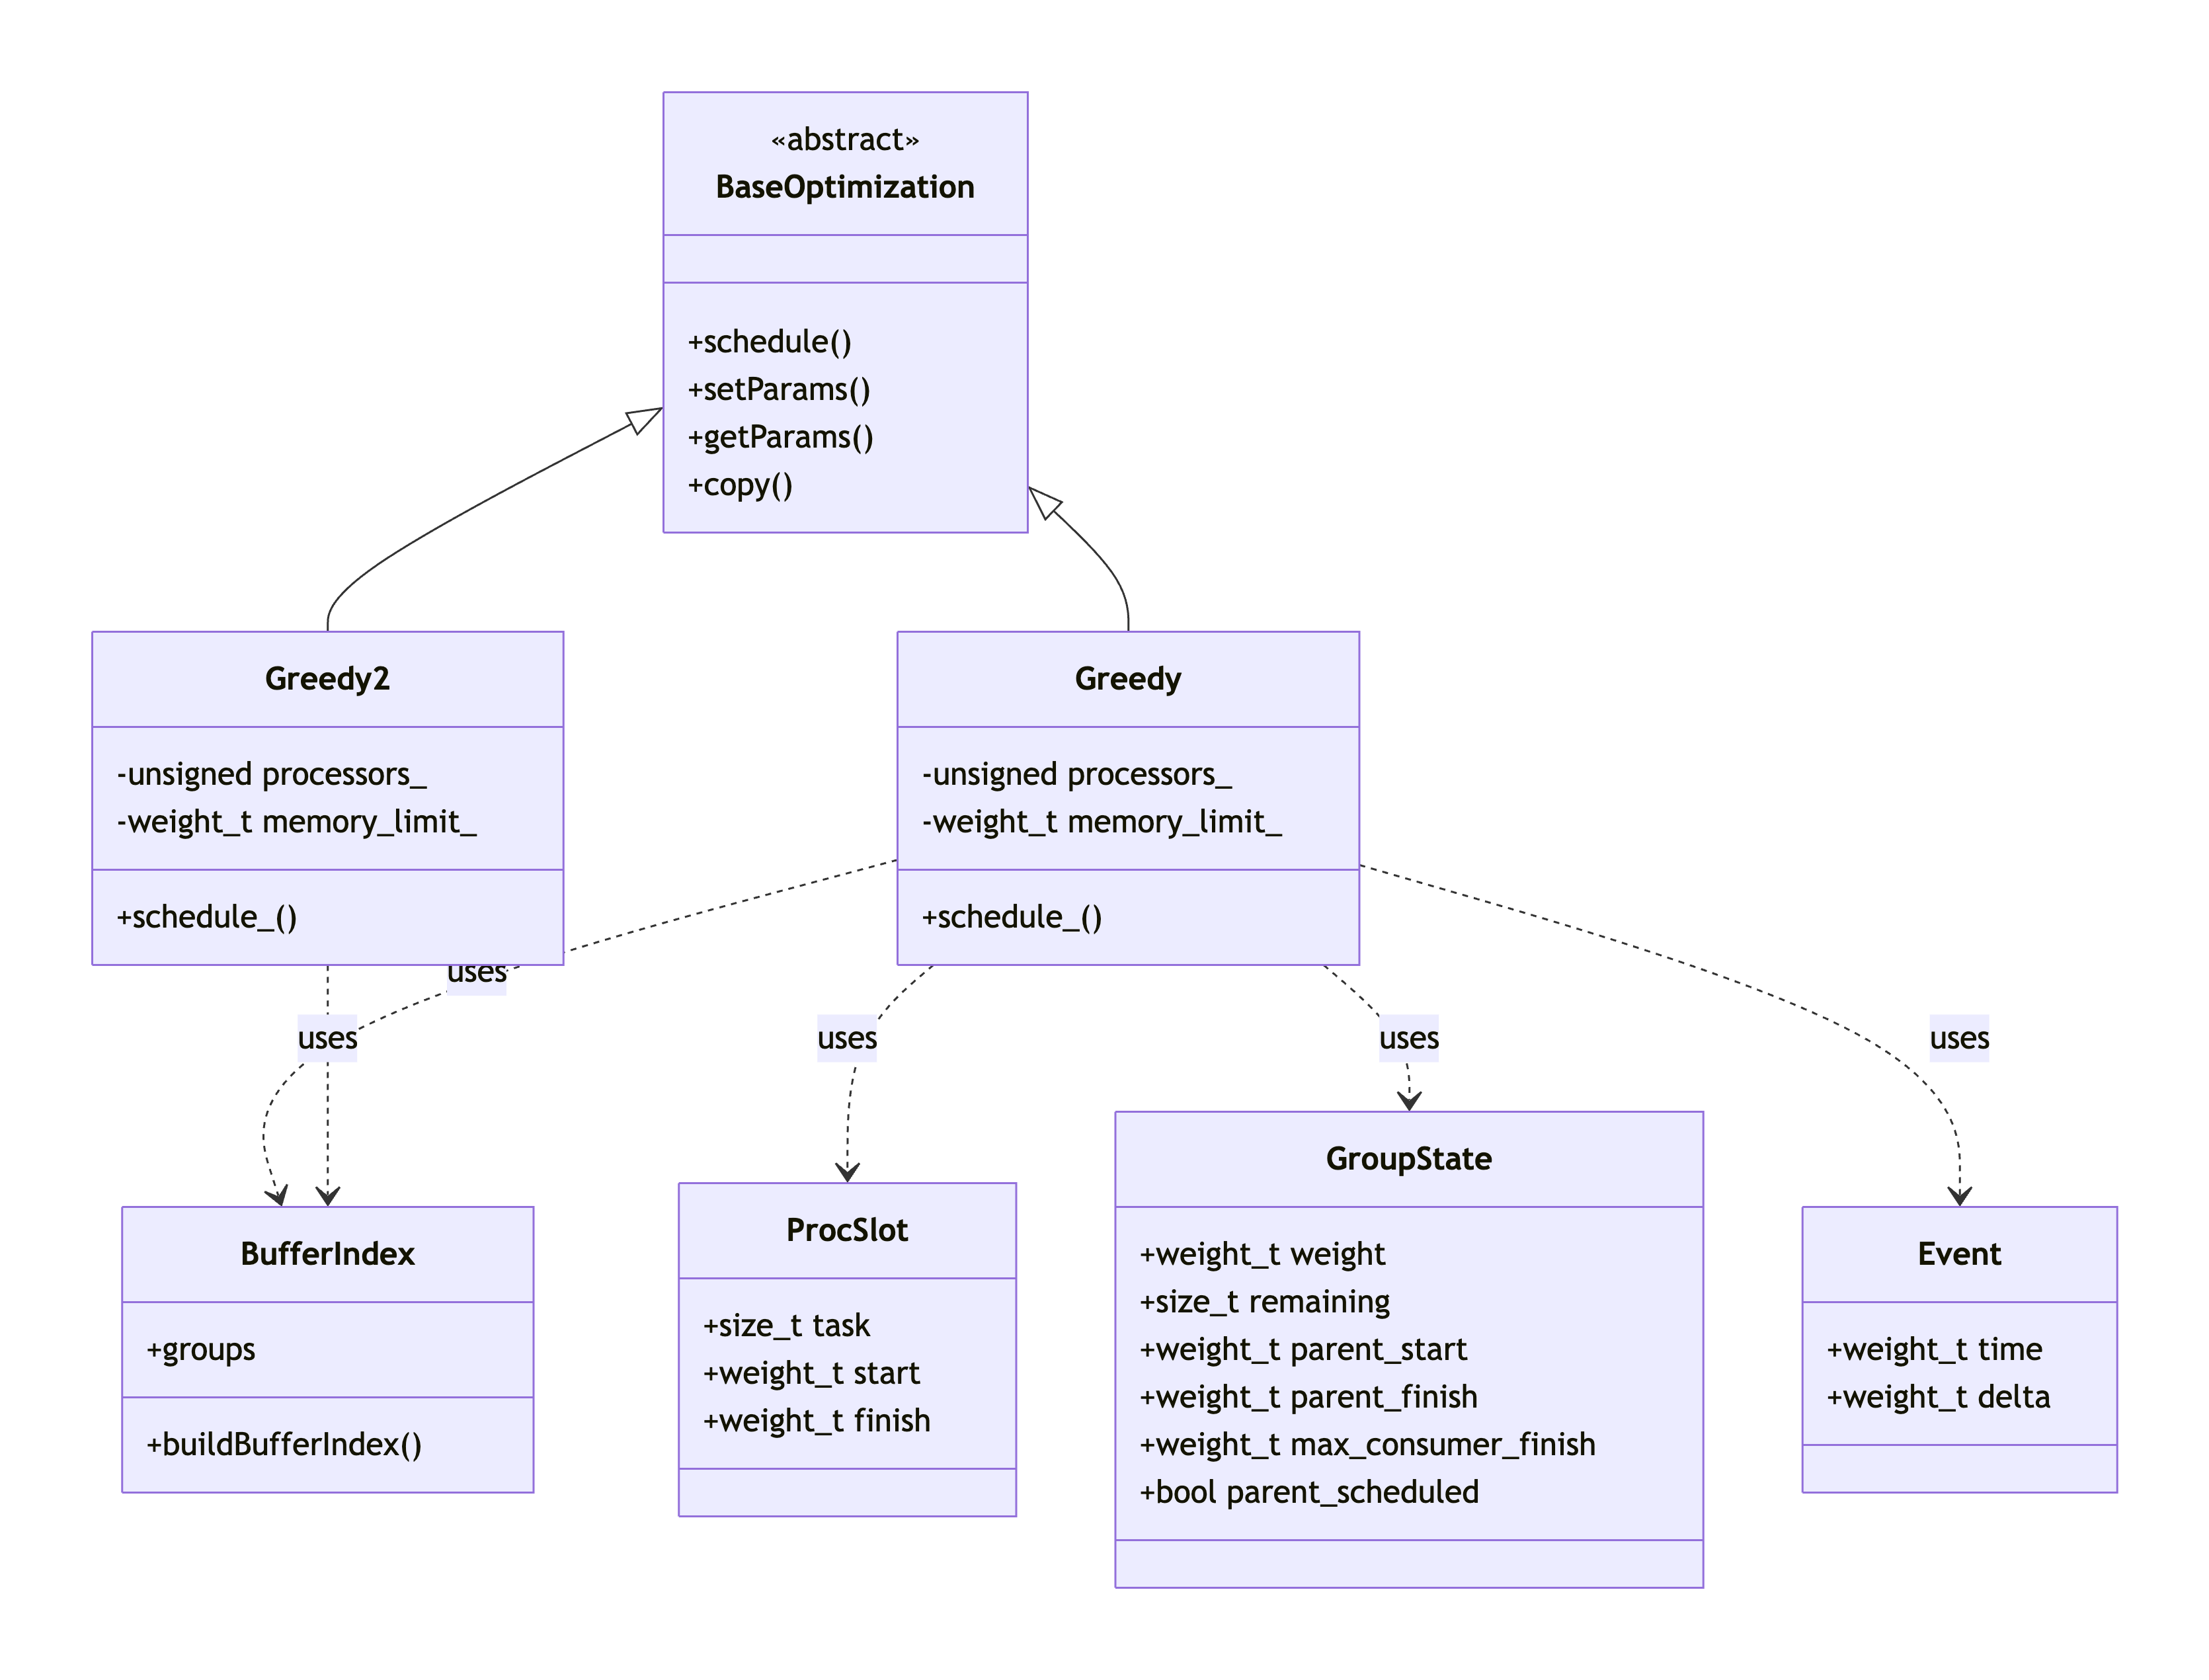
\includegraphics[width=1\textwidth]{pictures/greedy_class_diagram.png}
	\caption{Диаграмма классов жадного алгоритма}
	\label{fig:greedy_class_diagram}
\end{figure}

\paragraph{Базовый класс \texttt{BaseOptimization}}
Абстрактный класс, задающий интерфейс для всех алгоритмов оптимизации расписания. Содержит виртуальные методы \texttt{schedule()} (построение расписания), \texttt{setParams()}/\texttt{getParams()} (управление параметрами) и \texttt{copy()} (клонирование). Наследники должны реализовать конкретный метод \texttt{schedule\_()}.

\paragraph{Класс \texttt{Greedy} (EFT)}
Реализует жадный алгоритм, использующий эвристику \textbf{Earliest Finish Time (EFT)}. Ключевая функция — \texttt{earliestStartOnProcessor2()} — просматривает интервалы занятости процессора и находит подходящее окно.

\paragraph{Класс \texttt{Greedy2} (STS)}
Реализует эвристику \textbf{Smallest Time-Space (STS)}, учитывающую как длительность работы, так и её влияние на будущую занятость памяти. Вычисление оценки вынесено в отдельные переменные \texttt{output\_buffers\_weight\_sum} и \texttt{weighted\_duration\_sum} внутри основного цикла.

\paragraph{Вспомогательные структуры}
\begin{itemize}
	\item \texttt{ProcSlot} — описывает отрезок времени, занятый работой на процессоре (интервал $[start, finish)$).
	\item \texttt{GroupState} — состояние буфера: объём памяти, число оставшихся потребителей, время старта/завершения родительской работы и максимальное время завершения среди уже назначенных потребителей.
	\item \texttt{Event} — событие изменения занятости памяти (выделение или освобождение), используется при проверке допустимости по памяти.
	\item \texttt{BufferIndex} — индекс буферов, построенный по входному графу: для каждой работы хранит список её буферов, а для каждого буфера — список потребителей и объём. Используется для инициализации состояний \texttt{GroupState}.\\
\end{itemize}

\paragraph{Особенности реализации}
\begin{itemize}
	\item Все времена и объёмы памяти представлены целочисленным типом \texttt{weight\_t} (псевдоним \texttt{long long}).
	\item Процессоры нумеруются с 0 до $P-1$, расписание на каждом процессоре хранится как отсортированный вектор интервалов \texttt{ProcSlot}.
	\item Множество готовых работ поддерживается в \texttt{std::set} (автоматическая сортировка по идентификатору).
	\item Для ускорения поиска стартового окна на процессоре используется линейный проход по интервалам — в силу того, что число интервалов на процессор не превышает числа работ, а общее число работ редко превышает несколько тысяч, этого достаточно.
\end{itemize}

\subsection{Реализация подхода на базе ЦЛП}\label{sec:real_ILP}

Подход, описанный в разделе~\ref{sec:4_reduce_description}, реализован в виде набора скриптов на языке Python и Bash. Основные компоненты:

\begin{itemize}
	\item \texttt{make\_input\_times\_step2\_2.py} – транслятор, преобразующий входной граф работ в описание задачи ЦЛП на входном языке решателя SCIP (файл с расширением \texttt{.lp}).  
	Для каждого графа генерируется 10 упорядочений (см. подраздел~\ref{subsec:paral})
	Структура \texttt{.lp}-файла соответствует распределению, приведённому в табл.~\ref{tab:lp_sections}.
	
	\item \texttt{run\_many\_make\_inputs\_time\_for\_LP.py} – автоматизирует вызов транслятора для всех входных графов из каталога экспериментов. Из имени каждого файла извлекаются значения числа процессоров $P$ и лимита памяти $M$ (см. подраздел~\ref{subsec:datasets}), и эти параметры подставляются в глобальные переменные скрипта
	
	 \texttt{make\_input\_times\_step2\_2.py}.
	
	\item \texttt{run\_many\_solvers.py} – управляет выполнением серии экспериментов через обёрточный скрипт \texttt{run\_scip2.sh}. Ограничение времени работы решателя задаётся в файле \texttt{only\_time.set} (параметр \texttt{limits/time = 3600}).
	
	\item \texttt{run\_scip2.sh} – реализует параллельный запуск 8 экземпляров SCIP. Логи работы сохраняются в отдельные каталоги.
	
	\item \texttt{file\_reader\_and\_making\_json.py} – извлекает из логов SCIP значения переменных:
	\begin{itemize}
		\item $s_i$ (время старта работы $i$),
		\item $p_{ri}$ (номер процессора, назначенного работе $i$),
		\item вычисляет длительность как $\max_i (s_i + d_i)$.
	\end{itemize}
	Результат записывается в JSON-файл, полностью совместимый по структуре с выходными файлами жадных алгоритмов.\\\\\\
\end{itemize}

\begin{table}[ht]
	\centering
	\small
	\setlength{\tabcolsep}{4pt}
	\caption{Распределение переменных и ограничений по секциям \texttt{.lp}-файла}
	\label{tab:lp_sections}
	\begin{tabular}{|l|p{3cm}|p{6cm}|}
		\hline
		\textbf{Секция} & \textbf{Переменные / ограничения} & \textbf{Пояснение} \\
		\hline
		\texttt{Integer} & $l$, $s_i$, $\text{start}_{i,j}$, $\text{max\_end}_{i,j}$ & Целевая переменная, времена старта работ, начала и макс. завершения буферов \\
		\hline
		\texttt{Binary} & $m_{ij}$, $p_{ri}$, $t_{ij}$, $z_{ij}^{pq}$, $zz_{ij}^{pq}$, $a_{ij}^{pq}$, $aa_{ij}^{pq}$ & Отношения порядка, назначение на процессоры, пересечения буферов \\
		\hline
		\texttt{Subject to} & (\ref{eq:m_ge_frac})--(\ref{eq:m_le_frac}), (\ref{eq:prec}), (\ref{eq:no_conflict1})--(\ref{eq:no_conflict2}), (\ref{eq:z_start_new})--(\ref{eq:aa_end_new}) и др. & Основные линейные ограничения \\
		\hline
		\texttt{Bounds} & $m_{ii}=1$, $m_{ij}=1$ для $(i,j)\in E$ (включая транзитивные) & Фиксированные значения переменных предшествования \\
		\hline
		\texttt{Minimize} & $l$ & Целевая функция \\
		\hline
	\end{tabular}
\end{table}

Для генерации входных графов и подготовки наборов экспериментов использованы дополнительные скрипты:
\begin{itemize}
	\item \texttt{layered\_generator.py}, \texttt{random\_generator.py}, \texttt{triadag\_generator.py} – создают графы в «старом» формате (вершина, вес, список потомков) без учёта буферов.
	\item \texttt{converter.py} – преобразует «старые» графы в новый формат с буферами: назначает случайные длительности работ ($\in[10,100]$) и веса буферов ($\in[1,100]$), формирует два варианта группировки рёбер в буферы – один буфер (\texttt{\_1\_}) и равномерное корневое распределение (\texttt{\_N\_uniform\_}).
	\item \texttt{finding\_M\_and\_P.py} – для каждого полученного графа вычисляет на практике максимальное используемое число процессоров $P_{\max}$ и максимальную пиковую память $M_{\max}$ (при заведомо избыточных ресурсах). Затем создаёт 9 вариантов входных файлов ($3$ значения $P \times 3$ значения $M$) согласно сетке, описанной в подразделе~\ref{subsec:datasets}.
\end{itemize}

\subsection{Визуализатор временной диаграммы расписания}\label{sec:visual}

Для наглядного представления построенных расписаний (как полученных жадными алгоритмами, так и с помощью ЦЛП) разработан скрипт \texttt{gantt\_and\_memory.py} на языке Python с использованием библиотеки \texttt{matplotlib}. Он создаёт совмещённое изображение, состоящее из двух диаграмм:

\begin{enumerate}
	\item \textbf{Диаграмма Ганта} – отображает загрузку процессоров во времени. Каждая работа изображается цветным прямоугольником, внутри которого указан её идентификатор. По горизонтальной оси отложено время, по вертикальной – номера процессоров.
	\item \textbf{Диаграмма использования памяти} – показывает, как меняется суммарный объём занятой памяти в процессе выполнения расписания. По вертикальной оси отложен объём памяти, по горизонтальной – время. Дополнительно красной горизонтальной линией отмечается заданный лимит памяти $M$.
\end{enumerate}

\paragraph{Входные данные:}
\begin{itemize}
	\item JSON-файл с расписанием, содержащий для каждой работы номер процессора, время старта и завершения.
	\item Исходный TXT-файл графа работ в новом формате (с буферами), необходимый для определения, какие буферы активны в каждый момент времени.
\end{itemize}

\paragraph{Ключевые компоненты реализации:}
\begin{itemize}
	\item Функции рисования стрелок (\texttt{draw\_horiz\_arrow}, \texttt{draw\_vertical\_arrow},\\ \texttt{draw\_arc\_arrow}, \texttt{draw\_loop\_arrow} и др.) – используют \texttt{FancyArrowPatch} из\\ \texttt{matplotlib.patches}. Они проводят дуги и линии между работами, визуализируя зависимости по данным (рёбра графа). Тип стрелки зависит от взаимного расположения работ: горизонтальная, вертикальная, диагональная или дугообразная.
	\item Класс \texttt{ResourceVisualizer} – накапливает события изменения памяти (выделение и освобождение буферов) для каждого момента времени. Метод \texttt{visualize()} строит ступенчатую диаграмму, где каждый прямоугольник соответствует периоду активности конкретного буфера. Метод \texttt{add\_horizontal\_line()} добавляет линию заданного лимита памяти.
	\item Функция \texttt{get\_task\_coordinates} – вычисляет координаты работы на диаграмме Ганта по её времени старта, длительности и номеру процессора.
\end{itemize}

\paragraph{Выходные данные:}  
Скрипт отображает полученное изображение на экране (при интерактивном запуске) и может сохранить его в файл (например, в формате PNG) разрешением $300$ dpi.

Визуализатор активно используется при отладке алгоритмов, а также для качественного анализа полученных расписаний в ходе экспериментального исследования. С его помощью были построены, например, рисунки~\ref{fig:g6_greedy},~\ref{fig:g6_lp},~\ref{fig:EFT_20},~\ref{fig:lp_20}.

\subsection{Структура входного и выходного файлов}\label{sec:struct}

\subsubsection*{Входной файл (описание графа работ)}

Входной файл имеет расширение \texttt{.txt} и содержит строки в кодировке UTF-8.  
Первая строка является заголовком и содержит названия полей:
\begin{verbatim}
	id time weight_1: child_1 ... child_n, weight_2: child_1 ... child_n, ...
\end{verbatim}

Каждая последующая строка описывает одну работу (вершину графа) и имеет следующий формат:
\begin{verbatim}
	<id> <time> <буфер_1>, <буфер_2>, ..., <буфер_k>
\end{verbatim}
где
\begin{itemize}
	\item \texttt{<id>} — целочисленный идентификатор работы (от 0 до $n-1$);
	\item \texttt{<time>} — целочисленная длительность выполнения работы;
	\item \texttt{<буфер\_i>} имеет вид \texttt{<вес>: <список потомков>}, где \texttt{<вес>} — целое число, задающее объём памяти, занимаемый данным буфером, а \texttt{<список потомков>} — разделённые пробелами идентификаторы работ-потребителей этого буфера. Если у работы нет исходящих рёбер, в строке указывается единственный буфер \texttt{0:} (нулевой вес, пустой список потомков).
\end{itemize}

Буферы в строке разделяются запятой с пробелом (\texttt{`, `}). Внутри одного буфера после двоеточия может быть перечислено несколько потомков, что означает, что все они используют один и тот же буфер (и, следовательно, разделяют его данные). Пример строки для работы с двумя буферами:
\begin{verbatim}
	2   36   10: 3 6 7, 73: 4 8
\end{verbatim}
Это означает, что работа 2 длится 36 единиц времени, создаёт два буфера: первый весом 10 используется работами 3, 6, 7; второй весом 73 используется работами 4 и 8.

\subsubsection*{Выходной файл (расписание)}

Результат работы жадного алгоритма или решателя ЦЛП сохраняется в файл формата JSON с расширением \texttt{.json}. Файл содержит один объект, ключом которого является имя входного графа (без расширения), а значением — объект с полями, описывающими расписание. Структура JSON-объекта:

\begin{verbatim}
	{
		"имя_графа": {
			"makespan": целое,
			"runtime_sec": число с плавающей точкой,
			"size": целое,
			"schedule": {
				"id_вершины": {
					"processor": целое,
					"start": целое,
					"finish": целое
				},
				...
			}
		}
	}
\end{verbatim}

Поля означают:
\begin{itemize}
	\item \texttt{makespan} — общая длительность расписания (максимальное время завершения среди всех работ);
	\item \texttt{runtime\_sec} — реальное время работы алгоритма в секундах;
	\item \texttt{size} — число вершин в графе;
	\item \texttt{schedule} — словарь, где каждому идентификатору вершины соответствует словарь с тремя полями: \texttt{processor} — номер процессора (начиная с 0), на котором выполняется работа; \texttt{start} — время начала выполнения; \texttt{finish} — время завершения (\texttt{start} + длительность работы).
\end{itemize}
 
\anonsection{Заключение}
\label{sec:7_zakluch} \index{7_zakluch}

\singlespace

В результате выполнения работы получены следующие основные результаты:
\begin{enumerate}
	\item Разработан жадный алгоритм списочного планирования для многопроцессорной системы с ограничением на суммарный объём памяти. Реализованы две эвристики выбора работы: EFT (минимизация времени завершения работы) и STS (учёт затрат памяти на работу).
	\item Выполнено сведение задачи к задаче целочисленного линейного программирования (ЦЛП) с использованием переменных, моделирующих пересечение интервалов активности буферов. Реализовано построение расписания при помощи ЦЛП.
	\item Проведено экспериментальное исследование на трёх классах графов (слоистые, случайные, треугольные) размером от 10 до 990 вершин. Показано, что:
	\begin{itemize}
		\item ЦЛП находит оптимальное решение для всех малых графов с числом вершин не более 21, причем наибольшее преимущество у ЦЛП над лучшим из ЖА составляет более 32\%.
		\item При числе вершин больше 16 и малом числе доступных процессоров время работы ЦЛП приближается к лимиту 3600~с; для больших графов ЦЛП не применимо.
		\item Жадные алгоритмы работают на порядки быстрее, чем ЦЛП (миллисекунды–секунды). Среднее отклонение длительности ЖА от длительности ЦЛП составляет $9$–$13\%$, максимальное – до $35\%$.
		\item Сравнение эвристик EFT и STS показало, что STS лучше на треугольных графах и при больших ресурсах (числе процессоров, объеме памяти), но уступает EFT на случайных графах с малым числом процессоров. Рекомендуется запускать обе эвристики и выбирать лучшее расписание.
	\end{itemize}
\end{enumerate}

Направления дальнейших исследований включают:
\begin{itemize}
	\item поддержку целевых систем с процессорами различной производительности (длительность работы зависит от процессора);
	\item применение методов машинного обучения для выбора эвристики или предсказания «хороших» упорядочений переменных для ЦЛП;
	\item разработку гибридных алгоритмов, комбинирующих жадные эвристики и точные методы для графов среднего размера (50–200 вершин).
\end{itemize} 
\anonsection{Приложение}
\label{sec:8_appendix} \index{8_appendix}

Здесь будет приложение

\begin{center}
	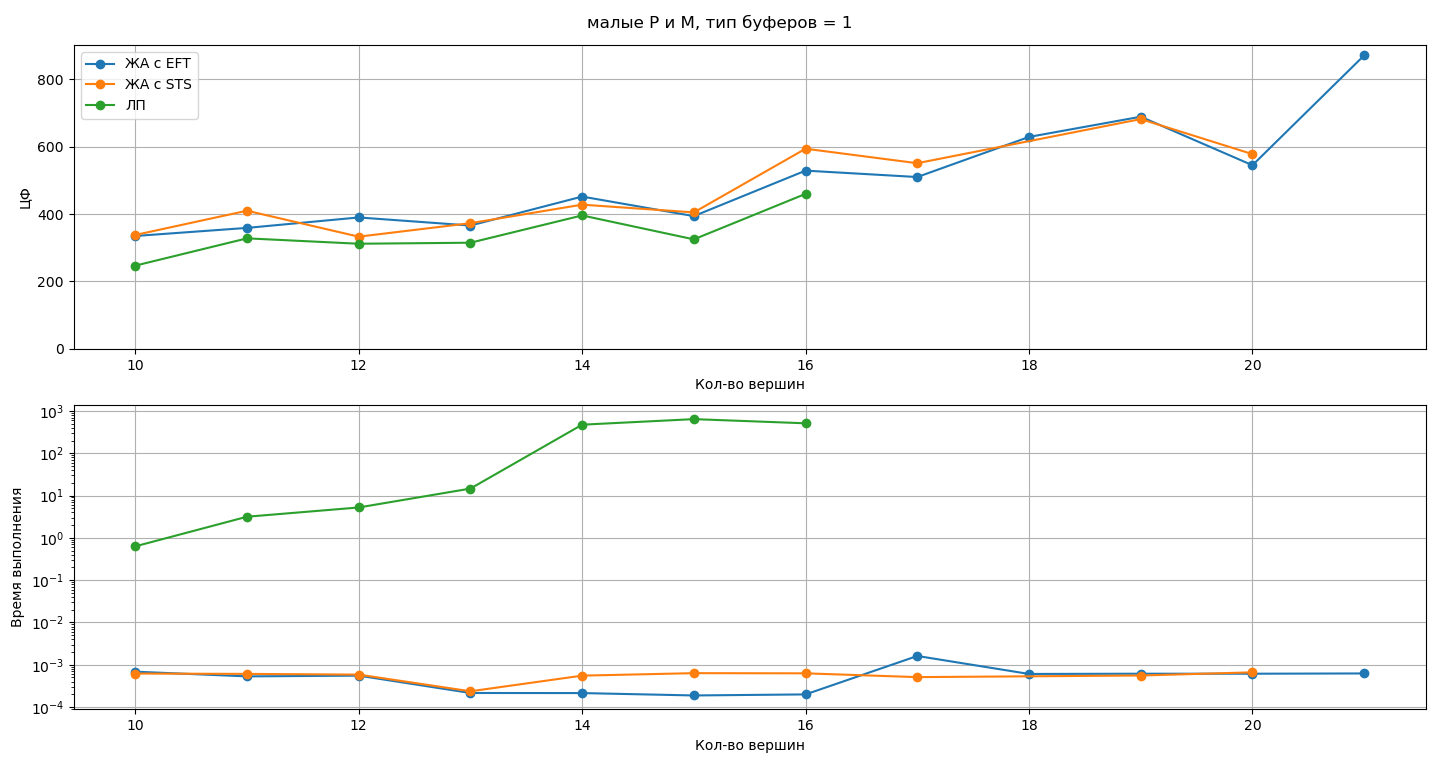
\includegraphics[width=1\textwidth]{pictures/low_P_and_M_1.png}
	\captionof{figure}{}
	\label{fig:scal1}
\end{center}

\begin{center}
	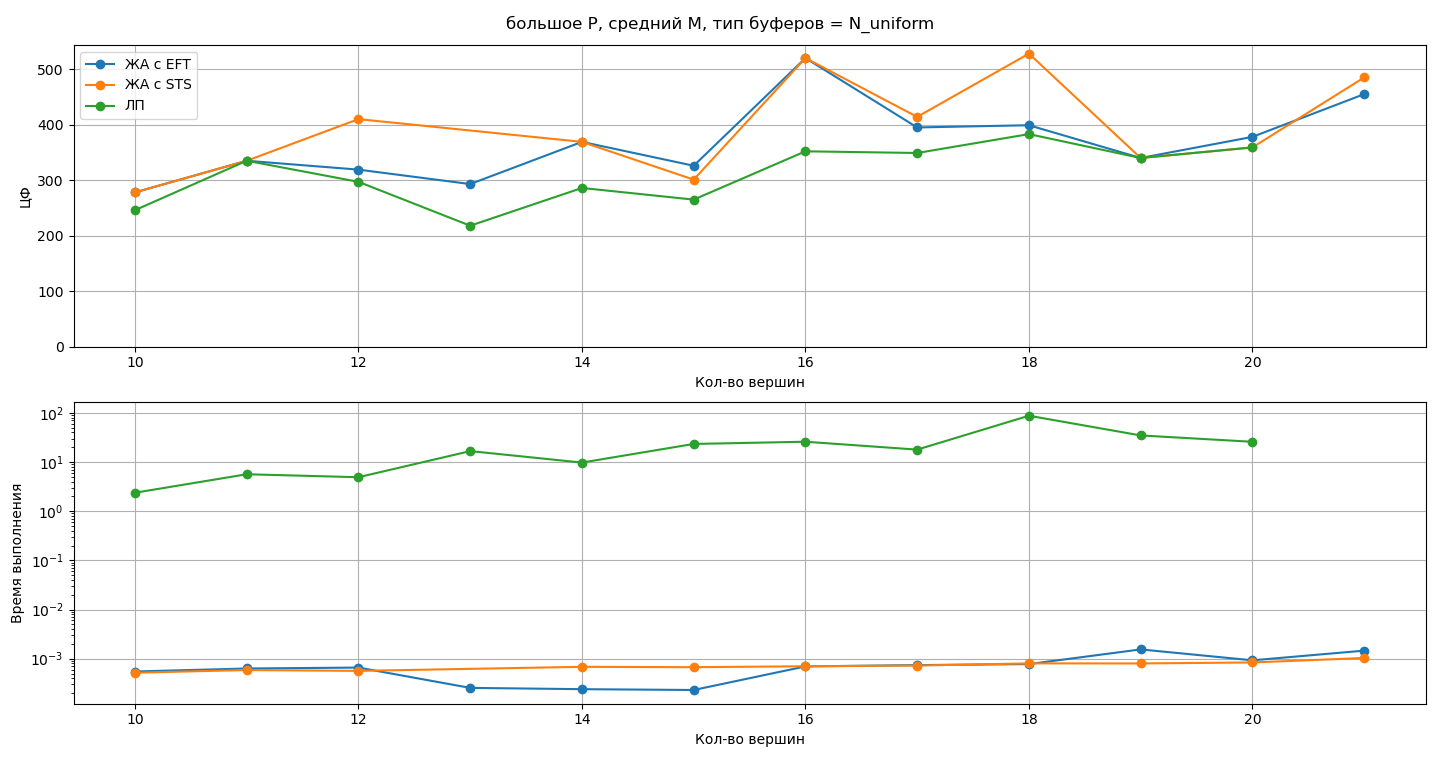
\includegraphics[width=1\textwidth]{pictures/high_P_mid_M_N_uni.png}
	\captionof{figure}{}
	\label{fig:scal4}
\end{center}

 На рисунке~\ref{fig:scal6} уже видно, что ЖА с STS не всегда завершается, в данном случае ему при любом числе процессоров не хватает минимального лимита памяти. На рисунке~\ref{fig:scal8} видно, как на графе с 15 вершинами уже долго работает ЛП при 2 доступных процессорах, но при этом всегда находит заметно лучшее расписание. На рисунке~\ref{fig:scal9} уже видно, что при 16 вершинах ЛП не завершается при P = 2. И на рисунке~\ref{fig:scal14} видно, как соотносятся алгоритмы на слоистом графе большого размера, видно, что там, где ЛП завершается, он часто дает заметно лучшее расписание по сравнению с ЖА. 

\begin{center}
	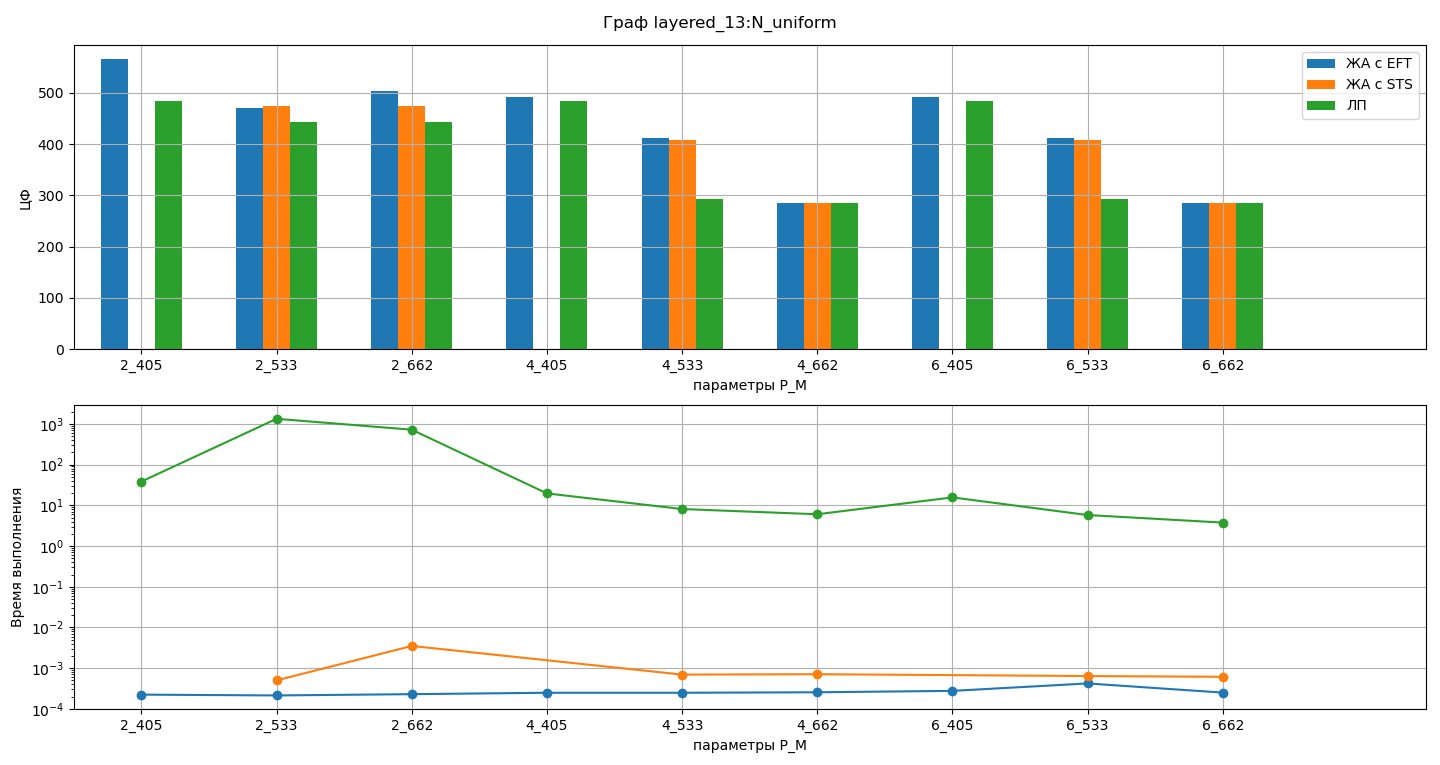
\includegraphics[width=1\textwidth]{pictures/layered_13_N_uni.png}
	\captionof{figure}{}
	\label{fig:scal6}
\end{center}

\begin{center}
	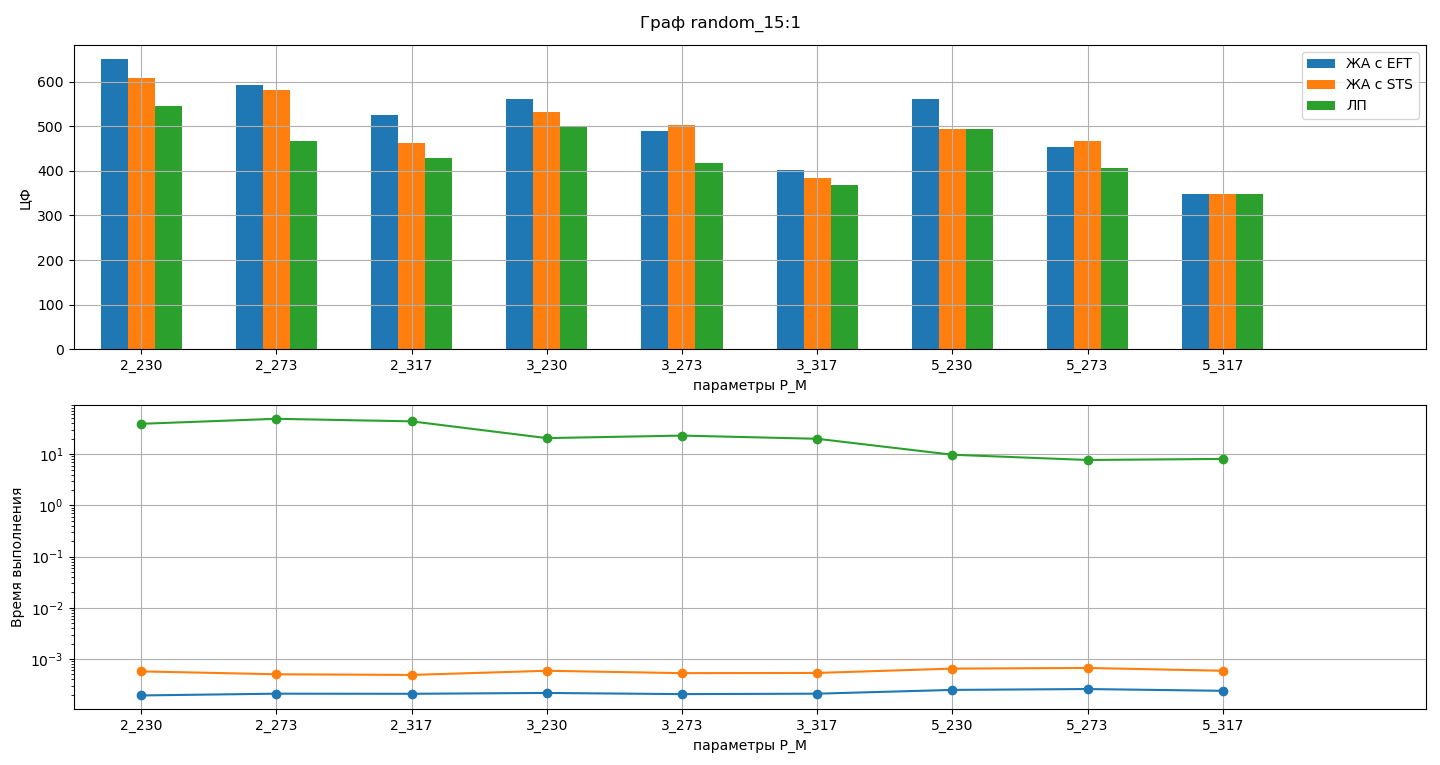
\includegraphics[width=1\textwidth]{pictures/random_15_1.png}
	\captionof{figure}{}
	\label{fig:scal7}
\end{center}

\begin{center}
	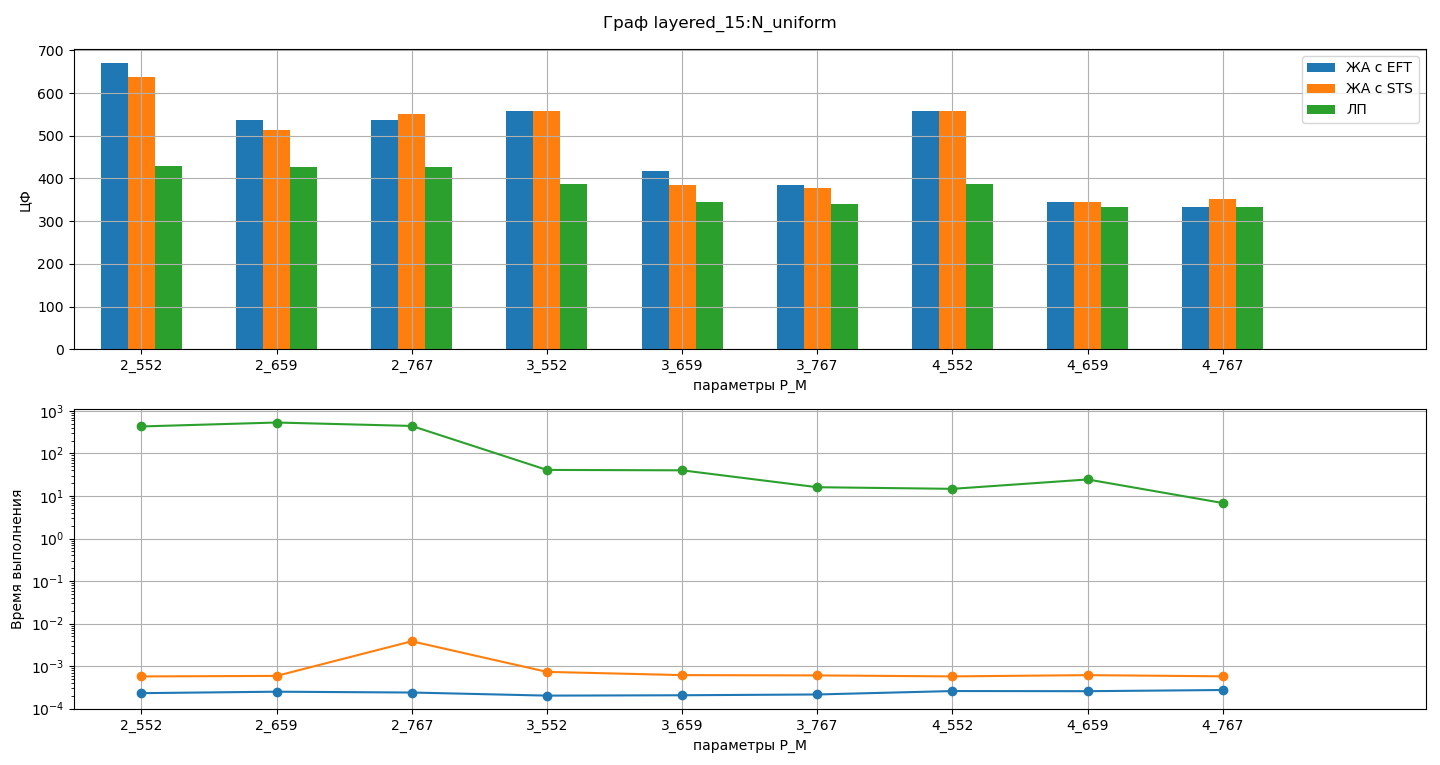
\includegraphics[width=1\textwidth]{pictures/layered_15_N_uni.png}
	\captionof{figure}{}
	\label{fig:scal8}
\end{center}

\begin{center}
	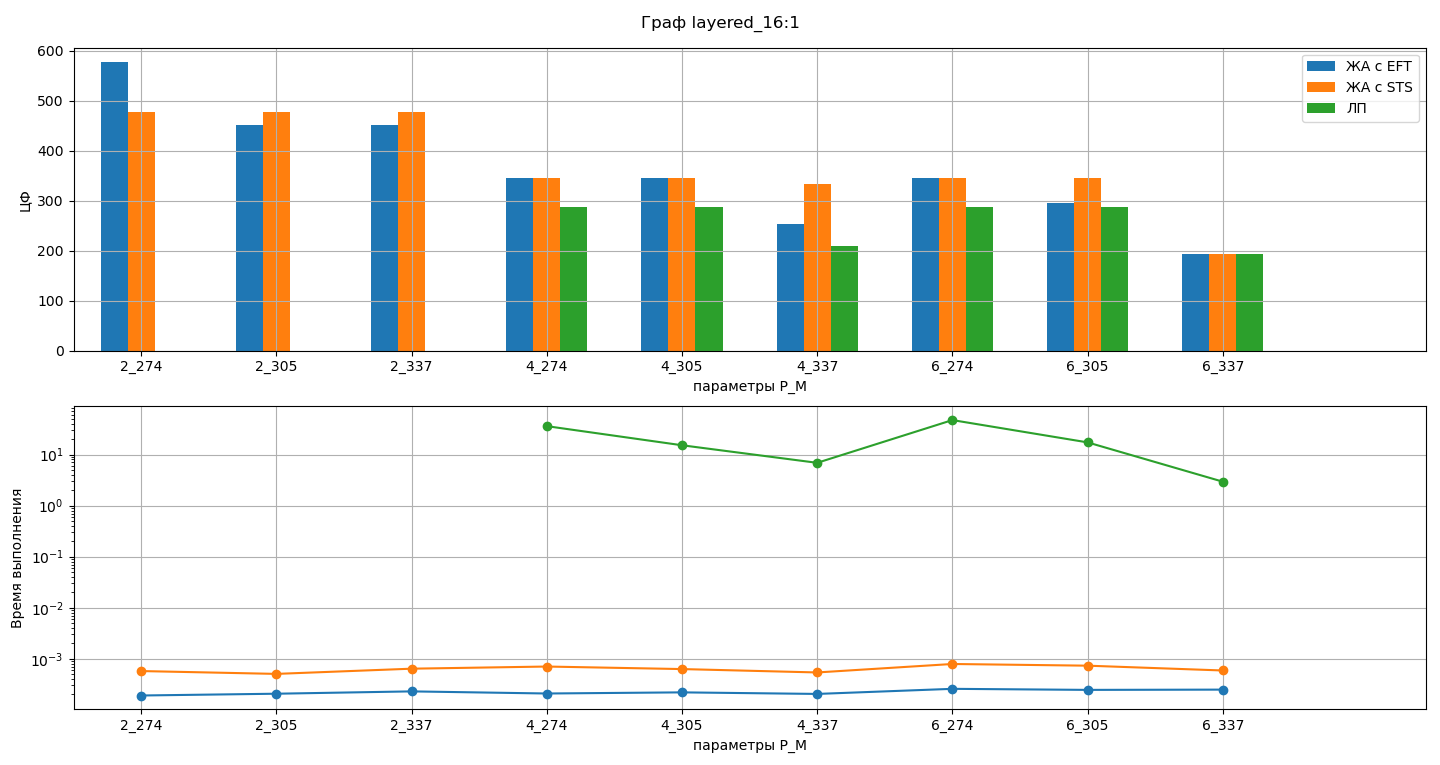
\includegraphics[width=1\textwidth]{pictures/layered_16_1.png}
	\captionof{figure}{}
	\label{fig:scal9}
\end{center}

\begin{center}
	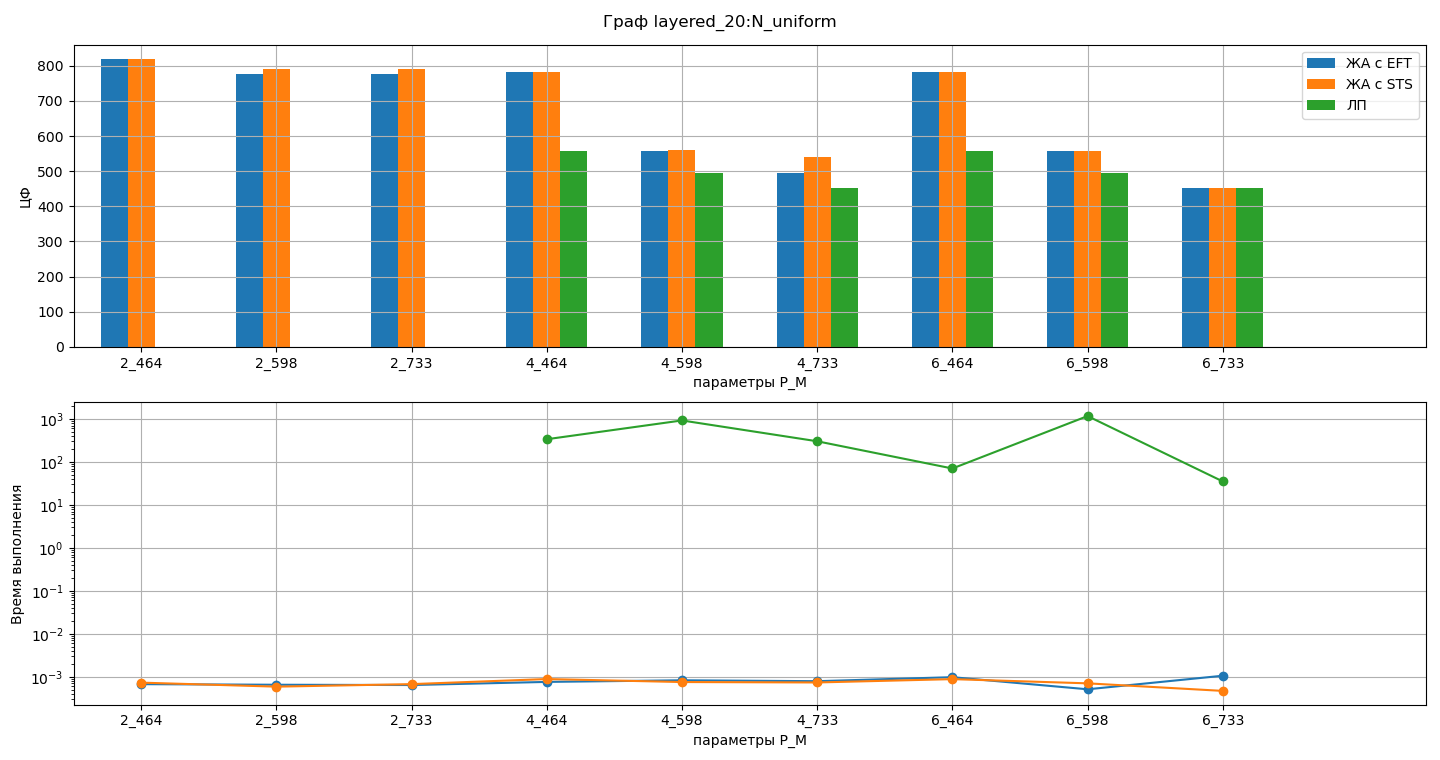
\includegraphics[width=1\textwidth]{pictures/layered_20_N_uni.png}
	\captionof{figure}{}
	\label{fig:scal14}
\end{center}


На рисунках~\ref{fig:EFT_12}-~\ref{fig:STS_12} видно, как ЖА с EFT может быть заметно лучше ЖА с STS, граф - layered\_12\_1\_2\_321. На рисунках~\ref{fig:EFT_16}-~\ref{fig:STS_16} видно обратную ситуацию, граф - layered\_16\_1\_2\_274. 

\begin{center}
	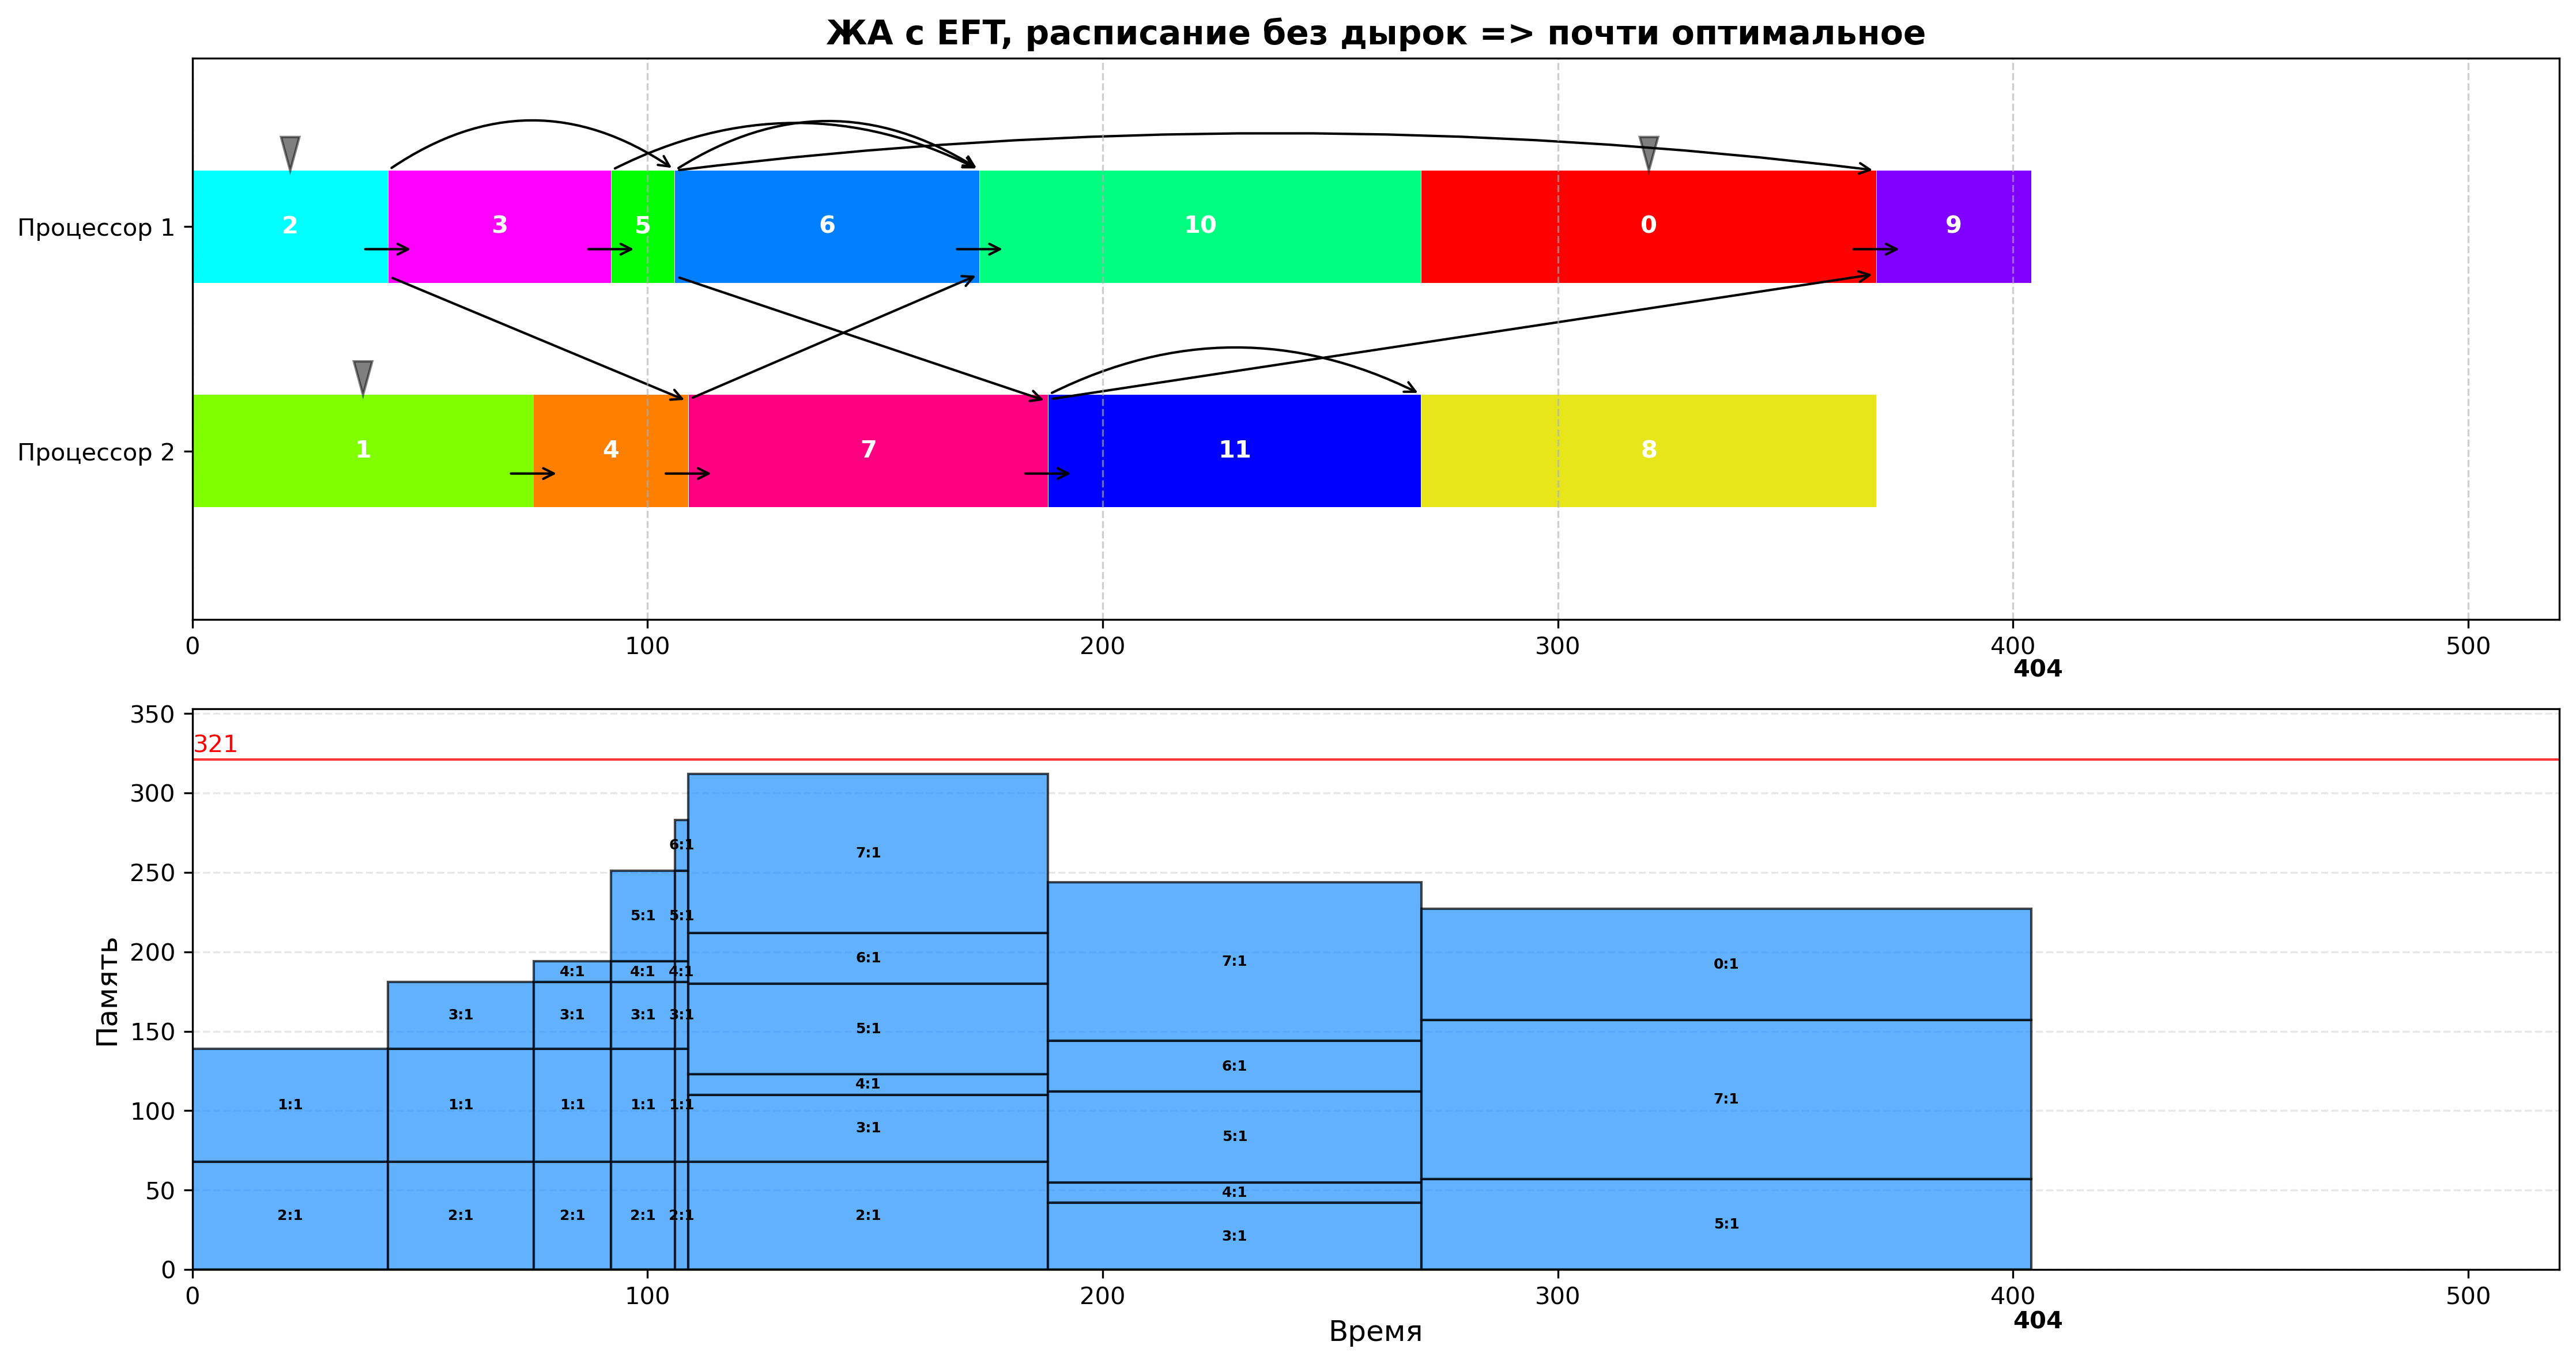
\includegraphics[width=0.8\textwidth]{pictures/greedy_EFT_layered_12_1_lp2_2_321.png}
	\captionof{figure}{}
	\label{fig:EFT_12}
\end{center}

\begin{center}
	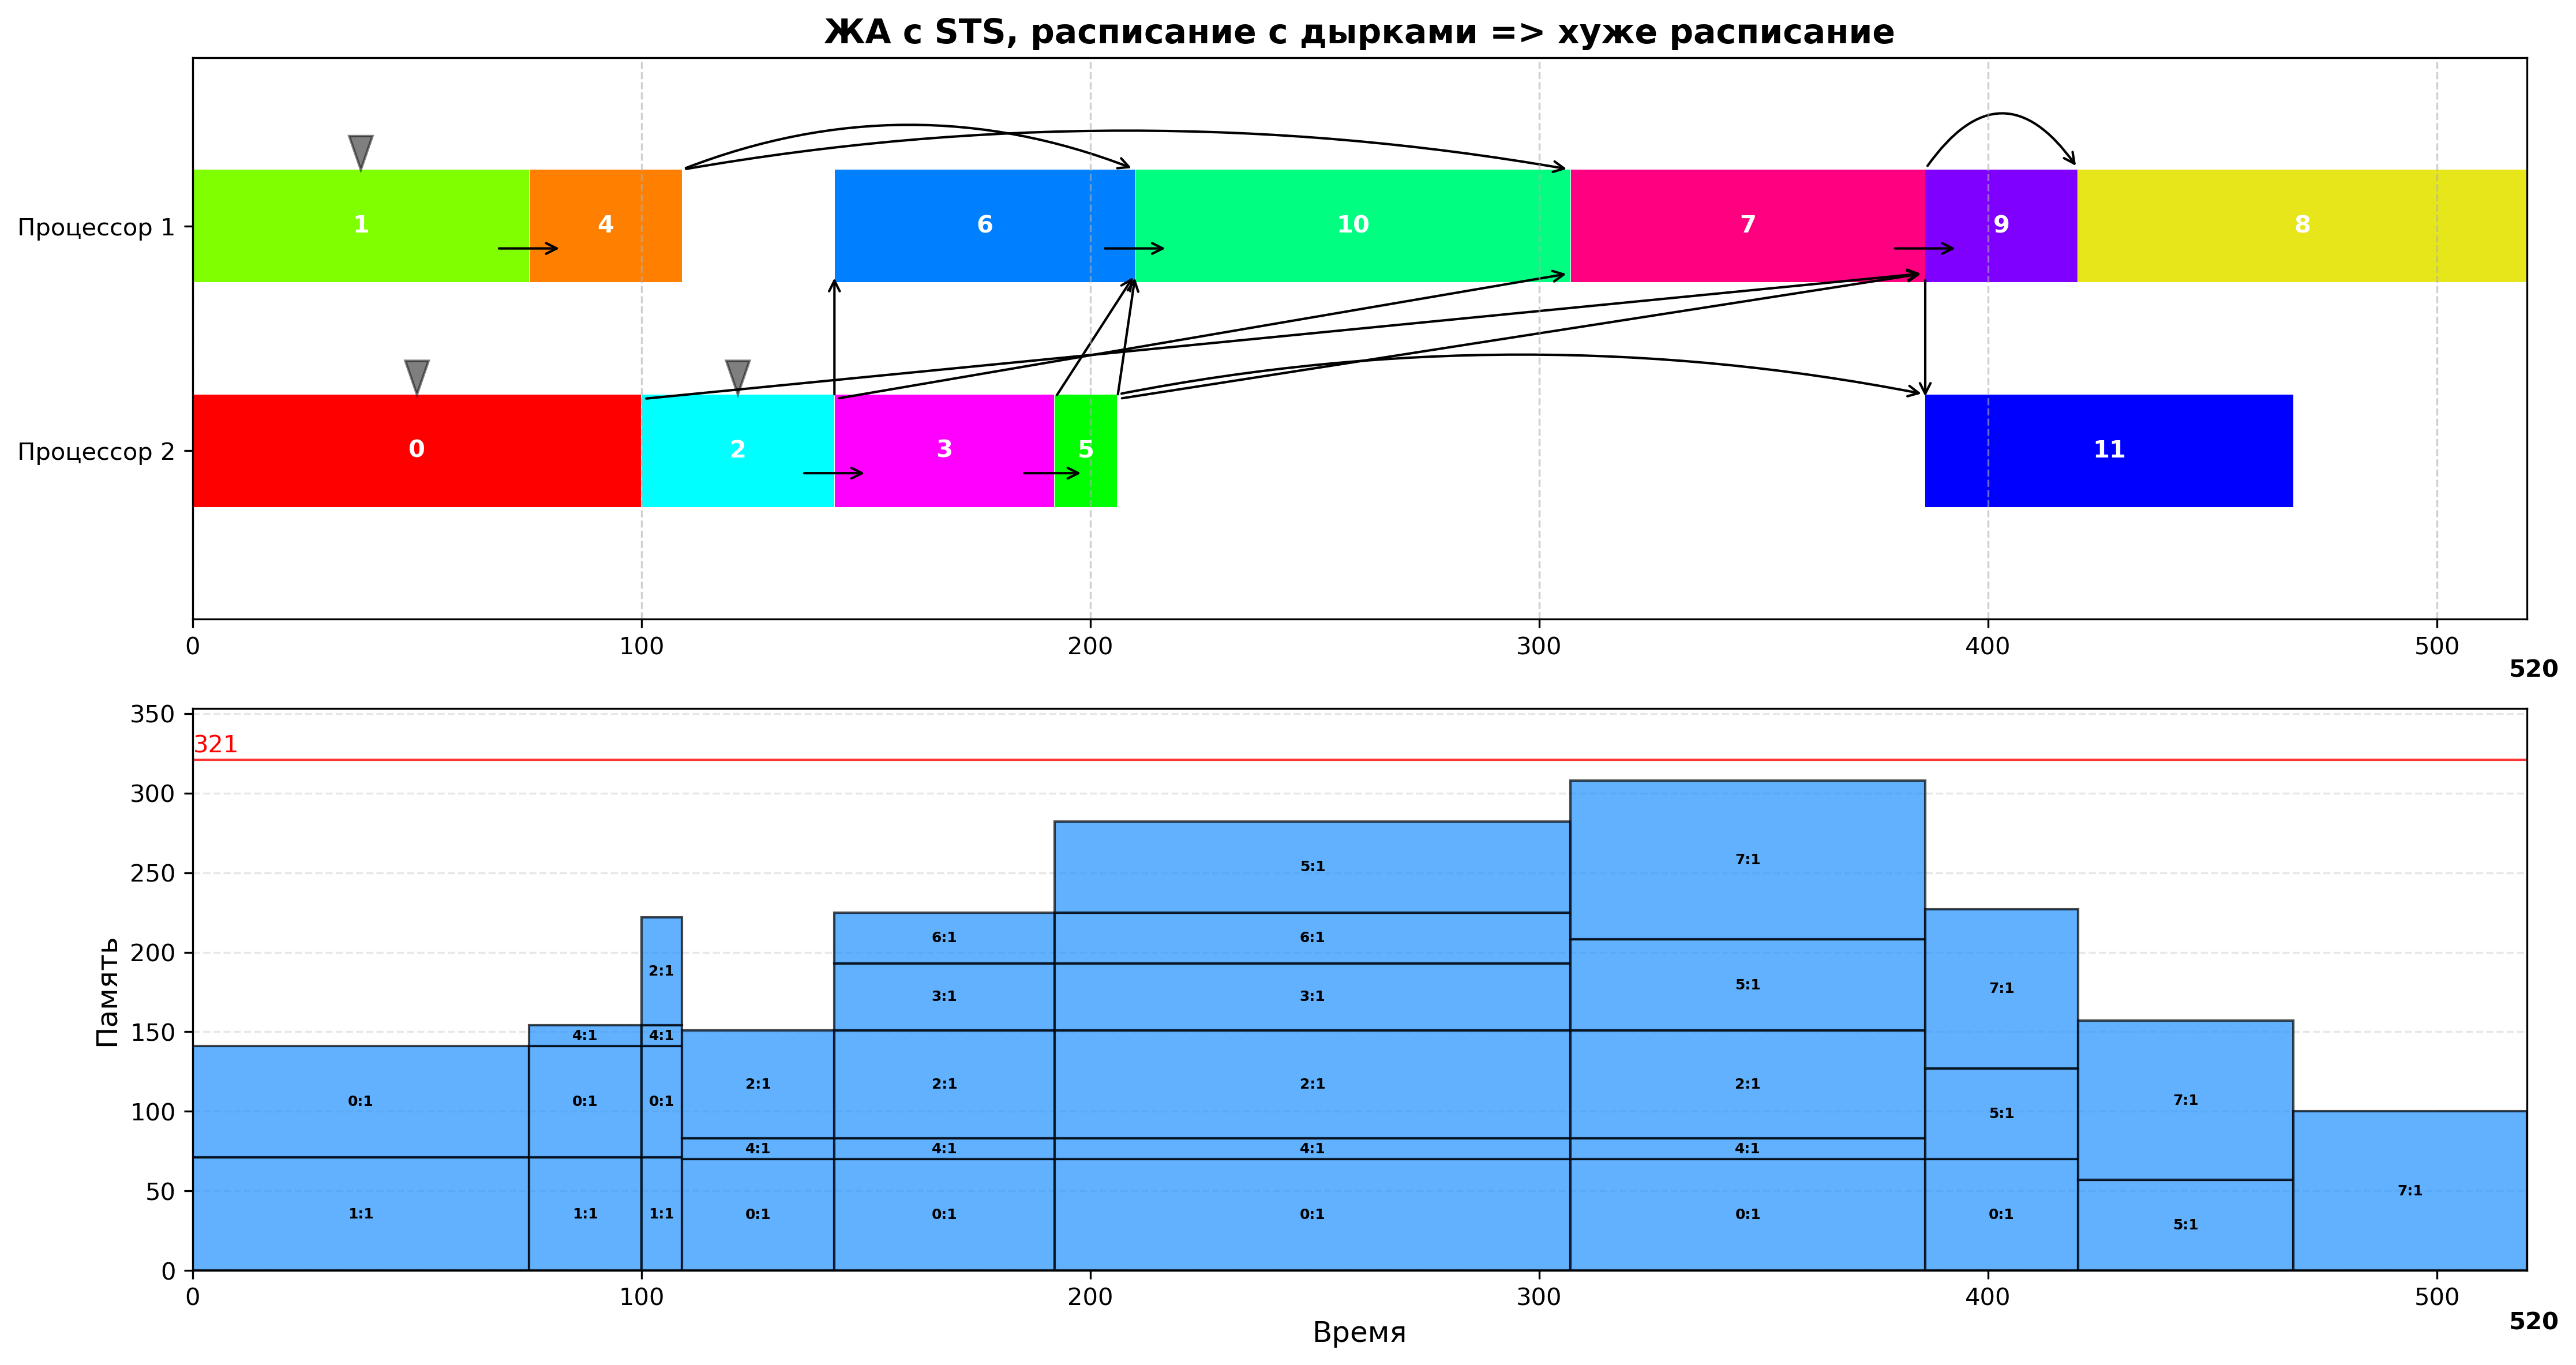
\includegraphics[width=0.8144\textwidth]{pictures/greedy_STS_layered_12_1_lp2_2_321.png}
	\captionof{figure}{}
	\label{fig:STS_12}
\end{center}

\begin{center}
	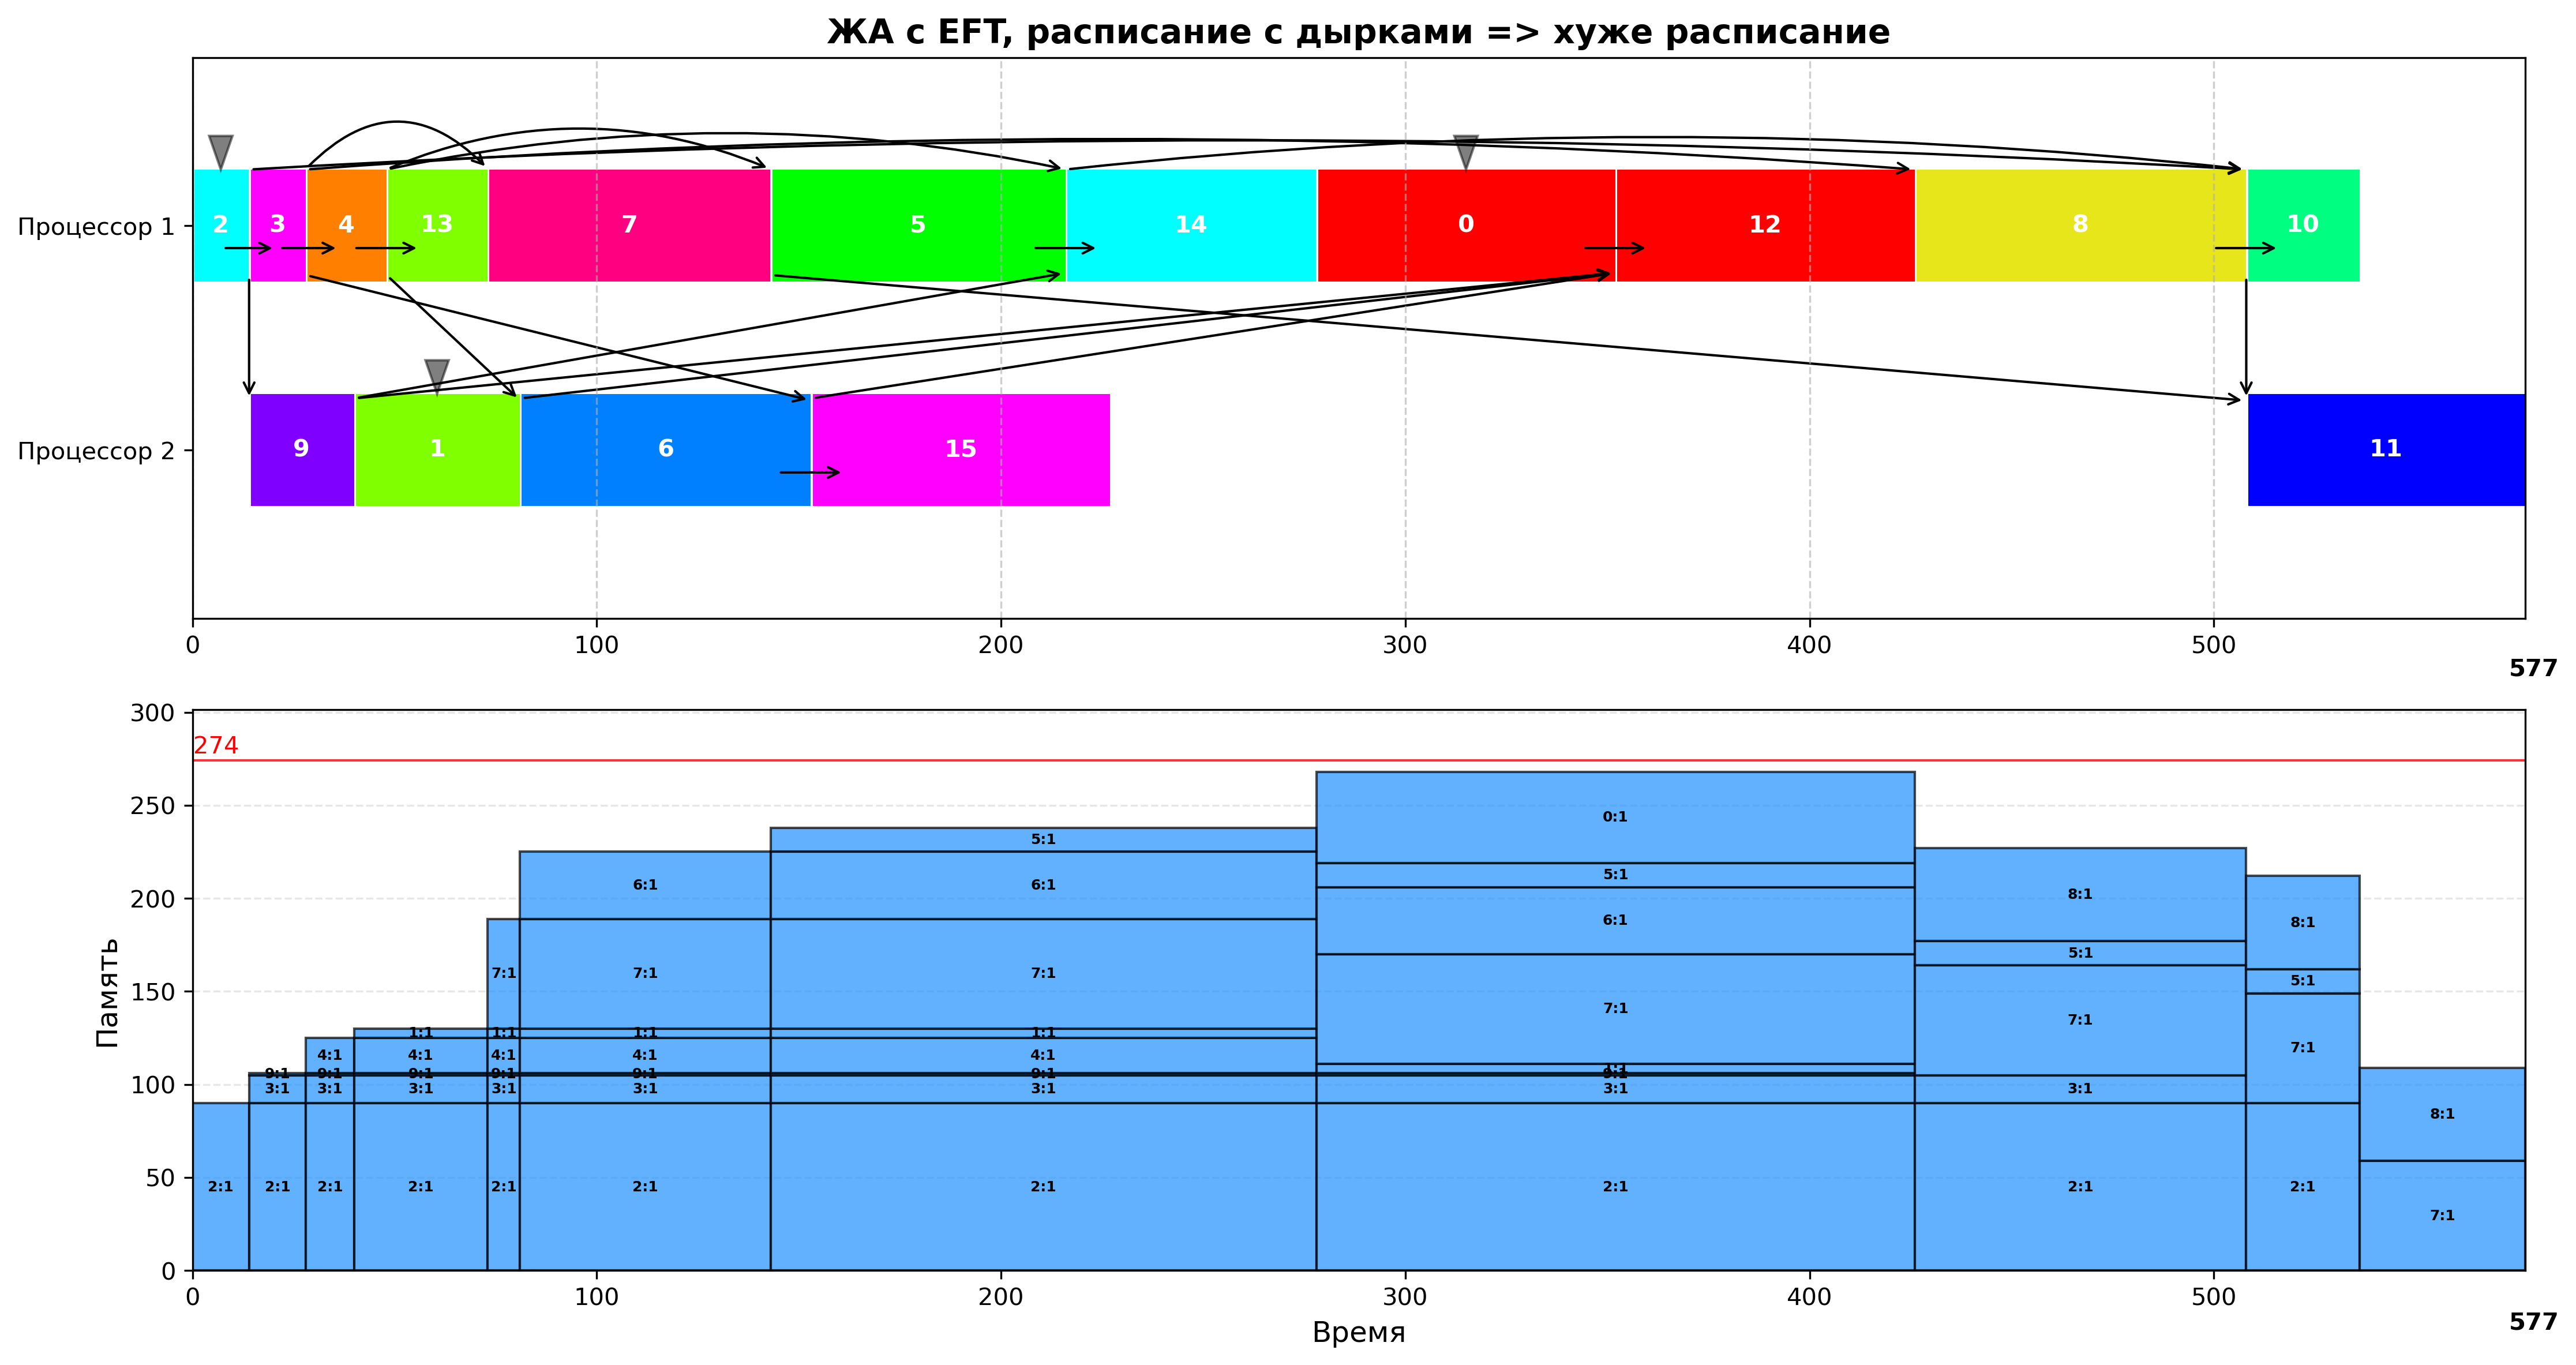
\includegraphics[width=1.018\textwidth]{pictures/greedy_EFT_layered_16_1_lp2_2_274.png}
	\captionof{figure}{}
	\label{fig:EFT_16}
\end{center}

\begin{center}
	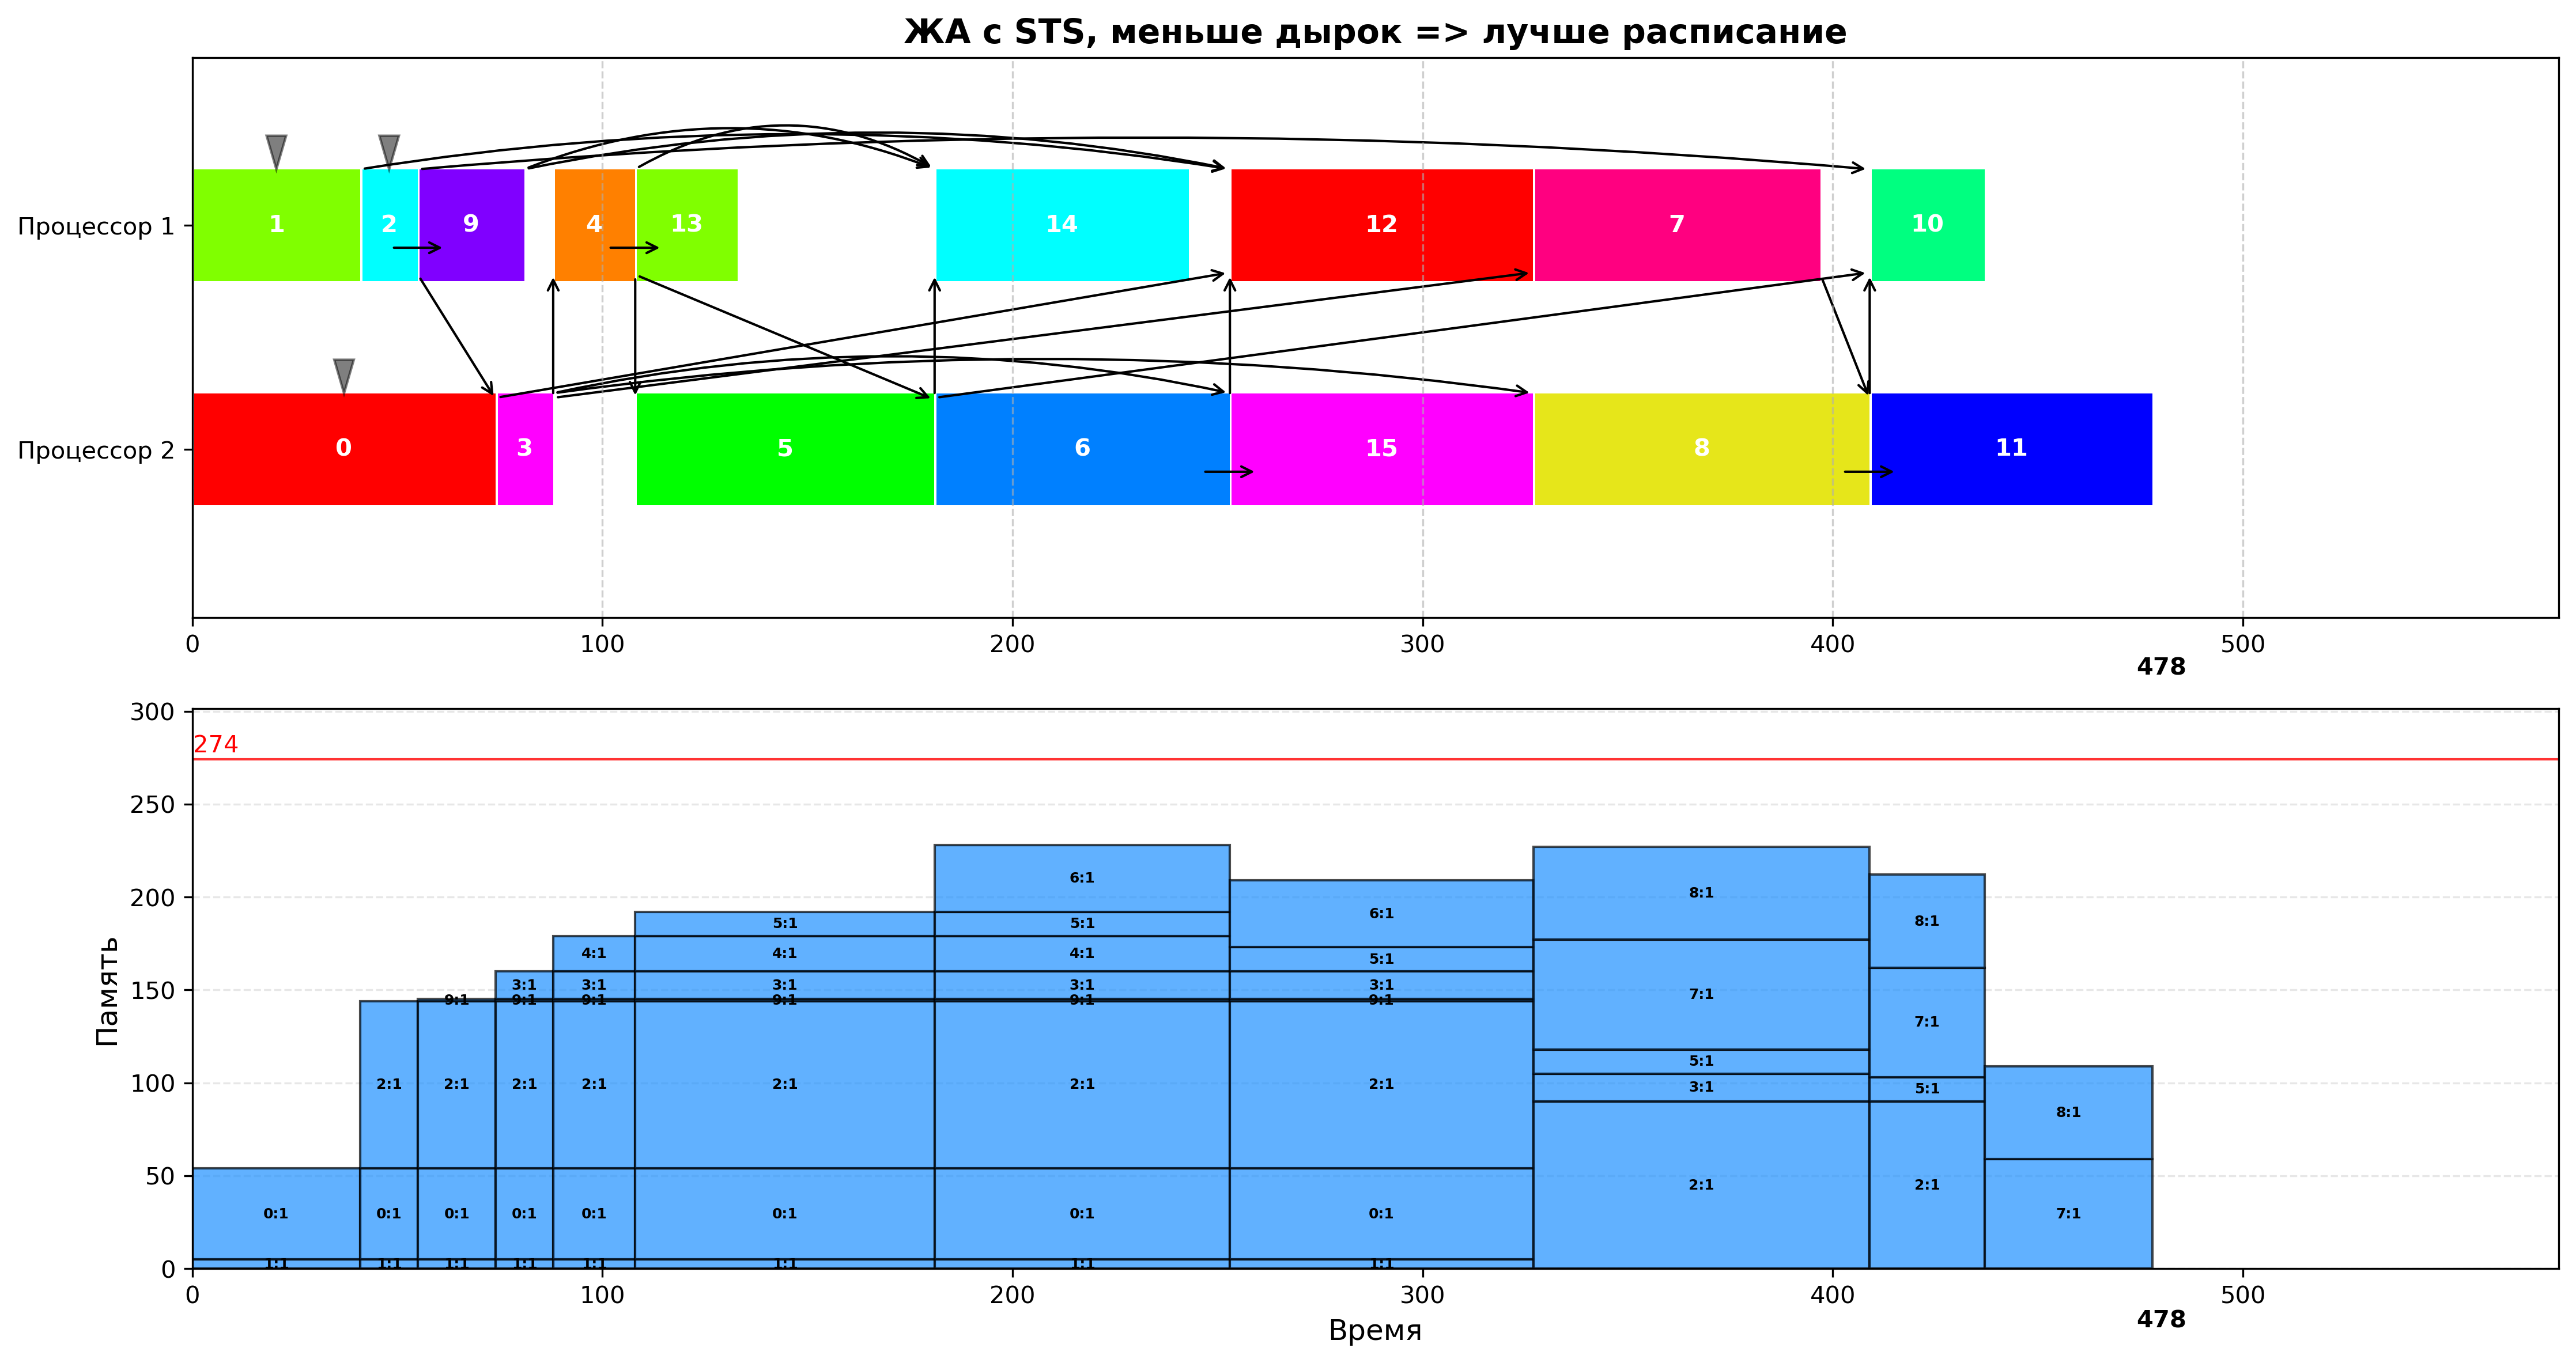
\includegraphics[width=1\textwidth]{pictures/greedy_STS_layered_16_1_lp2_2_274.png}
	\captionof{figure}{}
	\label{fig:STS_16}
\end{center}




\begin{center}
	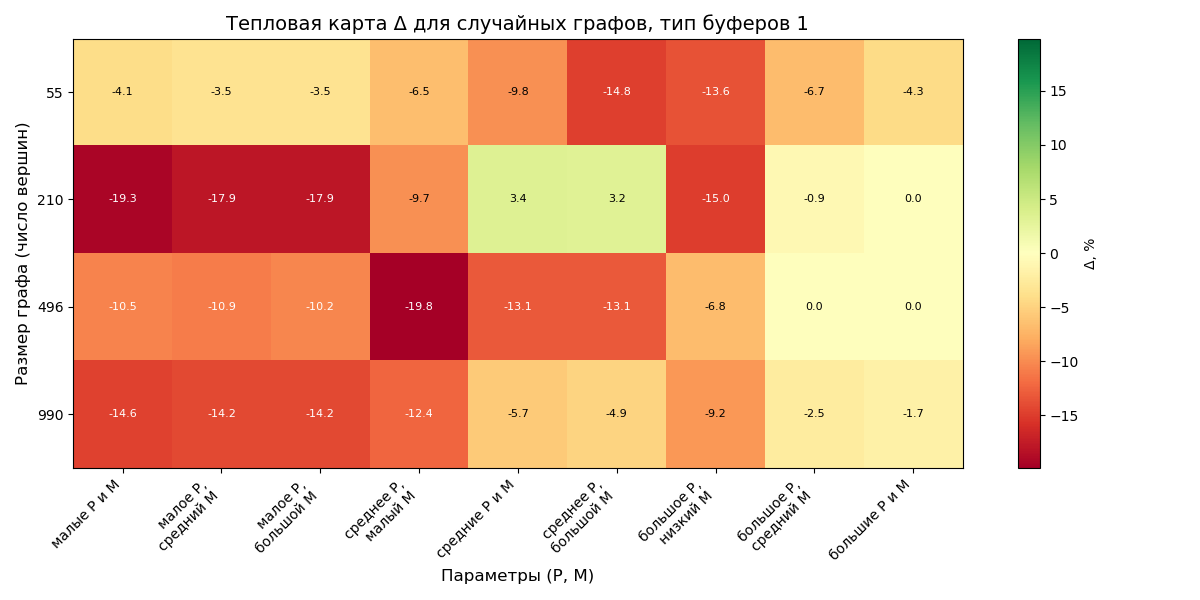
\includegraphics[width=1\textwidth]{pictures/heat_random_1.png}
	\captionof{figure}{}
	\label{fig:heat_rand}
\end{center}

\begin{center}
	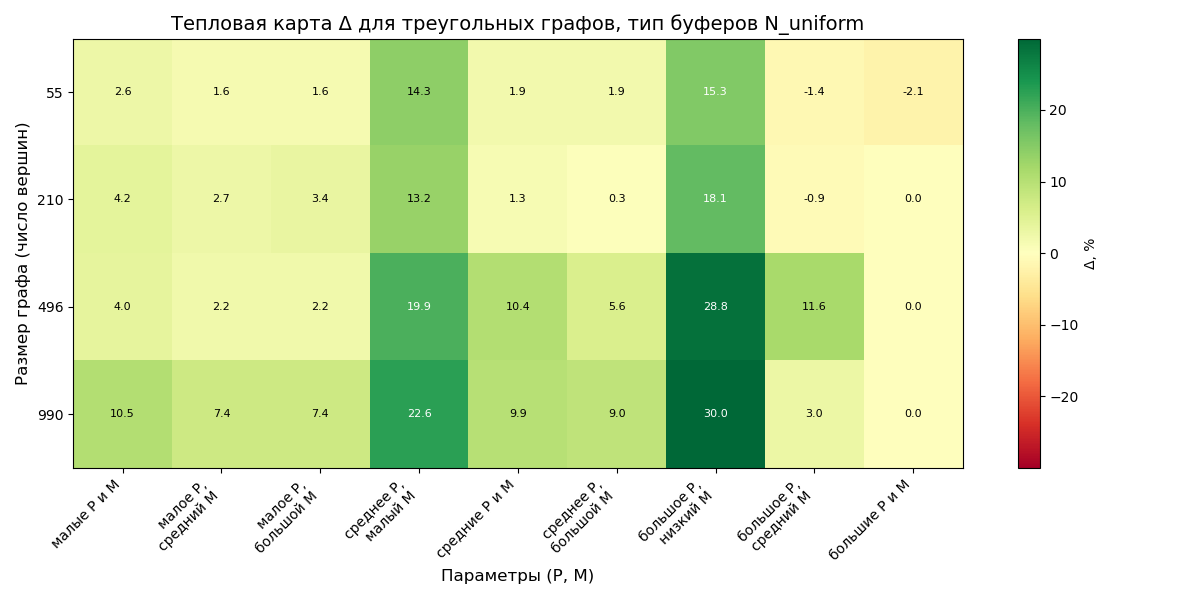
\includegraphics[width=1\textwidth]{pictures/heat_triadags_N_uni.png}
	\captionof{figure}{}
	\label{fig:heat_tri}
\end{center}
 
% \bibliographystyle{gost71u}
% \bibliography{references}


% \include{Appendix} 

\end{document}
